\chapter{Documento dei Requisiti Software}

\section{Glossario}
In questo capitolo vengono definiti i termini tecnici e i concetti chiave utilizzati all'interno della documentazione del progetto DietiEstates25. Lo scopo è fornire un riferimento univoco per facilitare la comprensione del dominio applicativo e delle funzionalità del sistema da parte di tutti gli stakeholder.

\begin{longtblr}
	[
	caption={Glossario dei termini},
	label={tab:glossario}
	]
	{
		hlines,
		vlines,
		row{even} = {bg=blue!10!white},
		row{1}={bg=azure3, fg=white, font=\sffamily},
		colspec = {lX},
		width = 0.85\linewidth,
		rowhead = 1
	}
	\textbf{Termine} & \textbf{Definizione} \\

	\texttt{Agente immobiliare} & Un professionista che lavora per conto di una agenzia immobiliare e che gestisce annunci immobiliari. \\

	\texttt{Amministratore} & Utente con privilegi elevati all'interno del gestionale della propria agenzia. \\
	
	\texttt{Cliente} & Un utente finale che utilizza il sistema per cercare annunci immobiliari. \\

	\texttt{Immobile} & Proprietà gestita dagli agenti immobiliari all'interno del sistema DietiEstates25. \\

	\texttt{Inserzione} & Annuncio di vendita o affitto di un immobile. \\

	\texttt{Mappa interattiva} & Strumento che permette la localizzazione e ricerca degli immobili. \\

	\texttt{Notifica} & Un messaggio inviato agli utenti (clienti o agenti immobiliari) per informarli di eventi significativi, come la prenotazione di una visita o il rifiuto di un appuntamento. Le notifiche vengono inviate via e-mail. \\

	\texttt{Ricerca avanzata} & Funzionalità che consente agli utenti di filtrare gli immobili per criteri multipli. \\
\end{longtblr}

\section{Modellazione target utenti}
Nel contesto della gestione immobiliare, interagiscono tre figure chiave, ognuna con esigenze e obiettivi specifici:

\begin{itemize}
	\item \textbf{Utente:} una persona interessata a trovare la casa ideale.
	
	\item \textbf{Agente immobiliare:} un professionista focalizzato sulla vendita e sulla gestione degli immobili.
	
	\item \textbf{Gestore agenzia:} una figura manageriale che coordina l’attività di un’agenzia immobiliare.
\end{itemize}

\subsection{Utente}

\begin{center}
	\begin{minipage}{.45\textwidth}
		\begin{tblr}
			{
				hlines,
				vlines,
				row{even} = {bg=blue!10!white},
				column{1}={bg=azure3, fg=white, font=\sffamily},
			}
			Nome & Lucia \\
			Cognome & Moretti \\
			Età & 25 anni \\
			Stato civile & Single \\
			Titolo di Studio & Laurea Magistrale in Informatica \\
			Professione & App developer \\
			Tratti personali & Calma, paziente, e simpatica \\
		\end{tblr}
	\end{minipage}
	\hfill
		\begin{minipage}{.25\textwidth}
		\begin{tikzpicture}
			\clip (0,0)  circle (2cm) ;
			\node[anchor=center] at (0,0) {
\includegraphics[width=6cm]{res/lucia_moretti}};
			%adjust this coordinate to move image
		\end{tikzpicture}
	\end{minipage}
\end{center}

\paragraph{Biografia}
Lucia Moretti, nata a Napoli il 12 aprile del 1999, lavora in Apple come UX/UI developer. Vive in periferia, ma il lungo tragitto per raggiungere l'ufficio l'ha spinta a cercare una casa più vicina al lavoro. Vorrebbe un appartamento moderno, ben collegato e con una buona efficienza energetica, per ridurre i costi.

\paragraph{Obiettivi}
Lucia desidera avere un appartamento in affitto vicino alla sede di lavoro. Cerca una buona piattaforma per trovare una casa fatta su misura delle sue esigenze senza dover non andare in un agenzia immobiliare tradizionale. Prima di fissare un appuntamento vuole avere una panoramica di tutti gli immobili che possano soddisfare le sue esigenze da programmatrice.

\paragraph{Interessi}
Lucia ama immergersi nella scrittura e nella lettura, e per lei la casa dei sogni è un luogo che ispira storie, con una biblioteca accogliente e un angolo perfetto per scrivere. Essendo una persona socievole, immagina una casa ideale con spazi ampi e accoglienti per ospitare amici e organizzare cene ed eventi, dove ogni ambiente trasmetta calore e convivialità. La sua passione per la tecnologia la porta a desiderare una casa intelligente, dotata di dispositivi innovativi e soluzioni smart che rendano la quotidianità più semplice ed efficiente, permettendole di dedicarsi alle sue passioni senza pensieri.

\paragraph{Frustrazioni e difficoltà}
Ogni giorno, Lucia si ritrova a scorrere decine di annunci online con foto ingannevoli e descrizioni vaghe, solo per scoprire che molte case sono già state vendute o affittate. Quando finalmente trova qualcosa di interessante, contattare proprietari o agenzie diventa una sfida: risposte che non arrivano, siti che chiedono sottoscrizioni ad abbonamenti, richieste economiche fuori dal suo budget.

\subsection{Agente immobiliare}
\begin{center}
	\begin{minipage}{.45\textwidth} 
		\begin{tblr}
			{
				hlines,
				vlines,
				row{even} = {bg=blue!10!white},
				column{1}={bg=azure3, fg=white, font=\sffamily},
			}
			Nome & Andrea \\
			Cognome & Rinaldi \\
			Età & 45 anni \\
			Titolo di studio & Geometra \\
			Professione & Agente immobiliare \\
			Stato civile & Sposato \\
			Tratti personali & Disponibile, introverso e riflessivo \\
		\end{tblr}
	\end{minipage}
	\hfill
	\begin{minipage}{.25\textwidth}
		\begin{tikzpicture}
			\clip (0,0)  circle (2cm) ;
			\node[anchor=center] at (0,0) {
\includegraphics[width=6cm]{res/andrea_rinaldi}}; 
			%adjust this coordinate to move image
		\end{tikzpicture}
	\end{minipage}
\end{center}
\paragraph{Biografia}
Nasce a Milano nel 28 Agosto del 1980. È un agente immobiliare con esperienza e una formazione da Geometra. È sposato e gestisce anche un'azienda agricola di famiglia. Sebbene apprezzi l'ordine e la sicurezza, trova frustrante la gestione degli appuntamenti e delle disdette dei clienti, preferirebbe un sistema più efficiente per organizzare il suo lavoro.

\paragraph{Obiettivi }
Andrea è un agente immobiliare dinamico e organizzato, sempre alla ricerca di strumenti che possano ottimizzare il suo lavoro e migliorare l’esperienza dei clienti. Il suo obiettivo principale è gestire in modo efficiente il suo portafoglio di immobili, inserendo facilmente dettagli fondamentali come numero di stanze, piano, presenza di ascensore, classe energetica e servizi disponibili. 

Per offrire una presentazione completa e coinvolgente, vuole poter visualizzare in un’unica piattaforma foto, video e informazioni dettagliate su ogni proprietà, comprese descrizione, prezzo e dimensioni. Inoltre, per garantire un servizio impeccabile, desidera ricevere notifiche automatiche sulle prenotazioni delle visite, così da organizzare al meglio il proprio tempo e offrire un supporto puntuale ai clienti.

\paragraph{Frustrazioni/Difficoltà}
Andrea si infastidisce quando i clienti cambiano o disdicono continuamente gli appuntamenti, chiamandolo ripetutamente in ufficio. Durante i periodi di maggiore afflusso, poi, diventa ancora più difficile gestire tutto con un’agenda cartacea.
I continui slittamenti o cambiamenti degli appuntamenti gli fanno perdere facilmente traccia delle prenotazioni e degli orari disponibili, creando confusione e aumentando lo stress.

\paragraph{Interessi}
Andrea non è solo un agente immobiliare determinato, ma anche un imprenditore che gestisce con dedizione un’azienda di famiglia. La sua esperienza nel settore agricolo lo ha reso estremamente attento alle necessità dei clienti, motivo per cui cerca strumenti digitali che gli permettano di mantenere un’organizzazione impeccabile anche nel suo lavoro immobiliare. 

Per lui, un’app che gli consenta di inserire facilmente tutti i dettagli degli immobili e monitorare ogni fase della vendita è essenziale per garantire efficienza e precisione. Sempre orientato al raggiungimento dei migliori risultati, Andrea trova particolarmente utile poter stare in stretto contatto con i propri clienti, così da non perdere nessuna opportunità e dimostrare la sua superiorità nel mercato immobiliare.

\subsection{Gestore di una agenzia immobiliare}
\begin{center}
		\begin{minipage}{.45\textwidth}
		\centering
		\begin{tblr}
			{
				hlines,
				vlines,
				row{even} = {bg=blue!10!white},
				column{1}={bg=azure3, fg=white, font=\sffamily},
			}
			Nome & Marco \\
			Cognome & De Santis \\
			Età & 55 anni  \\ 
			Stato civile & Sposato\\
			Titolo di studio & Diploma di Liceo Classico \\
			Professione & Gestore di un'agenzia immobiliare \\
			Tratti personali & Ambizioso, pragmatico e tranquillo
		\end{tblr}
	\end{minipage}
	\hfill
	\begin{minipage}{.25\textwidth}
		\begin{tikzpicture}
			\clip (0,0)  circle (2cm) ;
			\node[anchor=center] at (0,-3) {
\includegraphics[width=6cm]{res/marco_de_santis}}; 
			%adjust this coordinate to move image
		\end{tikzpicture}
	\end{minipage}
\end{center}


\paragraph{Biografia}
Nasce a Firenze nel 30 ottobre del 1970. Crede fortemente nel digitale e per tale motivo vuole utilizzare un app che sia veloce nell’aggiornare i prezzi dei suoi immobili. Ama lavorare in movimento e vuole che l'app gli permetta di monitorare facilmente gli annunci dei suoi clienti ovunque si trovi.

\paragraph{Interessi}
Marco ama bilanciare al massimo lavoro e piacere, puntando a ottimizzare i processi aziendali per avere più tempo da dedicare alla propria vita sociale. Appassionato di commedia, ama citare film e programmi TV nelle conversazioni quotidiane, rendendo l’ambiente lavorativo più leggero e divertente. La sua energia si manifesta anche nelle attività sociali: è sempre entusiasta delle feste in ufficio e vede il networking come un’occasione per consolidare rapporti e creare nuove opportunità. Al centro dei suoi interessi ci sono le relazioni personali, e proprio per questo desidera delegare il più possibile, così da avere più tempo per amici e famiglia. La gestione e l’innovazione aziendale sono una sua grande passione, motivo per cui investe in strumenti digitali che rendano più efficienti le operazioni quotidiane della sua agenzia, permettendogli di automatizzare compiti ripetitivi e concentrarsi su ciò che conta davvero: godersi la vita.

\paragraph{Obiettivi}
Marco ha un obiettivo ben chiaro in mente: semplificare la gestione della sua agenzia senza rinunciare al controllo sulle operazioni. Per questo, è interessato a creare account per i suoi collaboratori, così da delegare attività operative e concentrarsi su aspetti strategici. Vuole poter monitorare le performance di vendita e i progressi dell’agenzia in tempo reale, direttamente dall’app, per essere sempre aggiornato anche mentre è in movimento. L’accesso immediato a report e statistiche dettagliate è fondamentale per analizzare il mercato e ottimizzare le strategie di vendita, senza dover passare ore davanti al computer. Per lui, la possibilità di controllare le vendite dei suoi immobili e visualizzare informazioni aggiornate in tempo reale tramite un’unica piattaforma digitale è essenziale, perché gli permette di gestire l’agenzia in modo efficiente e, al tempo stesso, godersi la vita senza vincoli.

\paragraph{Frustrazioni/difficoltà}
Marco è frustrato dalla quantità di burocrazia che deve gestire ogni giorno e teme che l’agenzia perda clienti a causa dei portali online, che offrono servizi sempre più veloci per cercare immobili. Ogni giorno si trova a fare i conti con contratti, documenti e normative che rallentano tutto. Inoltre, i clienti sono spesso indecisi e i proprietari sopravvalutano i loro immobili, mentre la concorrenza online sembra avere la meglio. Marco sente la pressione di dover tenere il passo con queste nuove tecnologie e teme che, se non cambia, l’agenzia possa restare indietro.

\section{Casi d'Uso e descrizione dei requisiti}

In questa sezione vengono elencati e descritti in dettaglio i requisiti del sistema \textsc{DietiEstates}, individuati durante la fase di prototipazione sulla base delle specifiche funzionali fornite dal committente.

L’obiettivo di questa fase è stato quello di tradurre le esigenze espresse in termini operativi concreti, definendo le funzionalità che il sistema dovrà offrire per soddisfare le aspettative degli utenti finali e garantire il raggiungimento degli obiettivi progettuali.

I requisiti identificati sono stati analizzati e formalizzati tenendo conto dell’ambiente operativo, dei vincoli tecnici e delle priorità indicate. Essi costituiscono la base per lo sviluppo del sistema e saranno utilizzati come riferimento per le attività di verifica, validazione e collaudo.

\begin{center}
	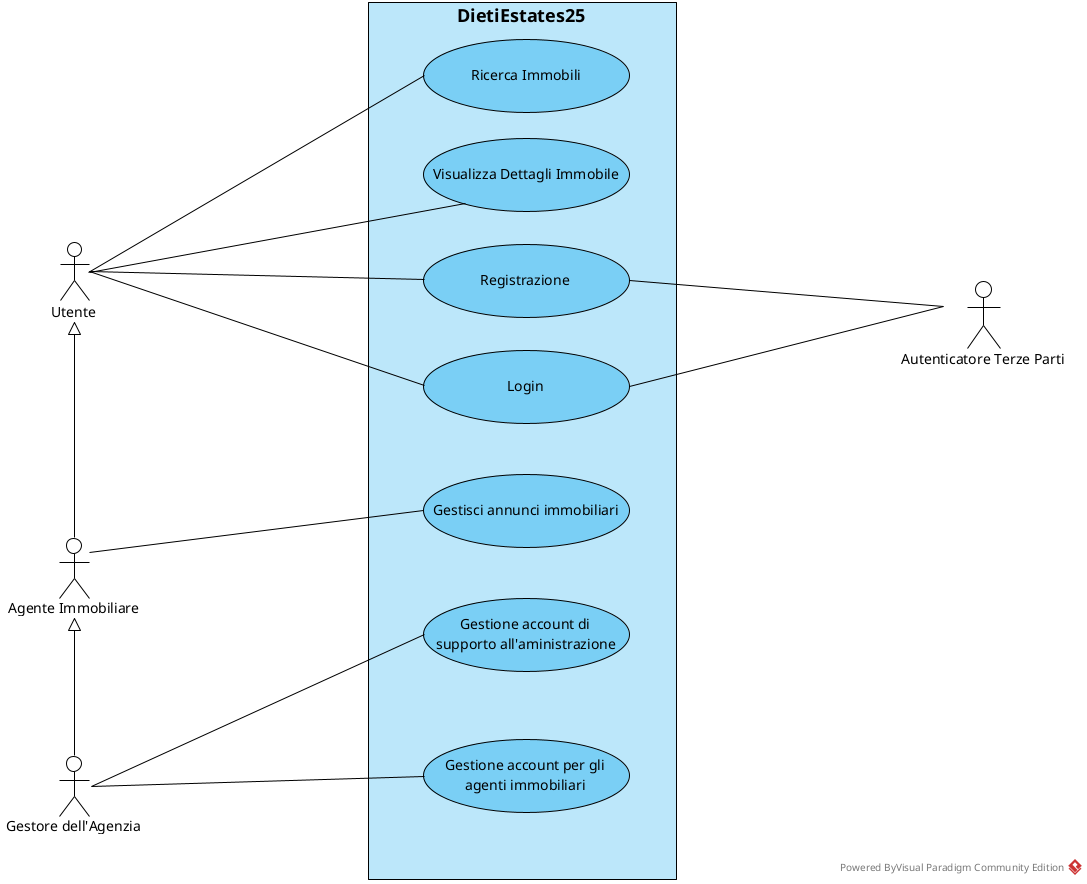
\includegraphics[width=\textwidth]{res/Use Case Diagram.png}
\end{center}

\subsection{Descrizione dei requisiti}
\begin{enumerate} 
	\item \textbf{Performance (Prestazioni):} 
	\begin{enumerate} 
		\item Il sistema deve essere performante, con tempi di risposta rapidi per garantire un'ottima esperienza utente. 
		\item Il motore di ricerca deve essere ottimizzato per gestire grandi volumi di annunci immobiliari, con tempi di elaborazione costanti.
	\end{enumerate}
	
	\item \textbf{Autenticazione, autorizzazione e gestione degli utenti} 
	\begin{enumerate} 
		\item Il sistema permette a più agenzie di pubblicare inserzioni immobiliari. Ogni installazione di \textsc{DietiEstates25} include un'utenza di amministrazione per il gestore dell'agenzia immobiliare, che viene creata con credenziali predefinite. Dopo aver effettuato l'accesso, è possibile modificare la password di amministrazione.
		\item Il sistema deve implementare un meccanismo di autenticazione sicura basato su token JWT (JSON Web Token), da includere nelle richieste alle API protette.
		\item Ogni utente è identificato univocamente da Nome, Cognome ed Email. L'indirizzo email è considerato \textbf{univoco} e utilizzato per l'autenticazione.
		\item Non è consentita la registrazione di più account con lo stesso indirizzo email. In caso di inserimento di un'email già registrata, il sistema deve notificare l'errore e impedire la creazione.
		\item Gli utenti sono associati a ruoli che definiscono le autorizzazioni sulle funzionalità del sistema. I ruoli previsti sono:
		\begin{itemize}
			\item \texttt{ADMIN}: amministratore di una agenzia immobiliare (gestione annunci e collaboratori);
			\item \texttt{AGENT}: collaboratore dell'agenzia immobiliare (gestione annunci, gestione appuntamenti);
			\item \texttt{USER} : utente generico che visualizza annunci e prenotare degli appuntamenti.
			\item \texttt{ADMIN\_ASSISTANT}: agente immobiliare con il privilegio di aggiunta, rimozione e promozione. 
		\end{itemize}  
		\item Gli agenti con ruolo \texttt{ADMIN} oppure \texttt{ADMIN\_ASSISTANT} hanno la facoltà di creare account per agenti immobiliari e di promuovere un (\texttt{AGENT}) al ruolo \texttt{ADMIN\_ASSISTANT}:
		\begin{itemize}
			\item Un agente con tale ruolo \textbf{non può} eliminare agenti con il ruolo \texttt{ADMIN} o auto-promuoversi a tale ruolo.
			\item Laddove l'email del nuovo agente immobiliare fosse già presente nel database, il sistema procede alla modifica del ruolo dell'account in questione.
			\item La promozione ad \texttt{ADMIN\_ASSISTANT} deve essere confermata con una doppia verifica da parte dell'amministratore.
			\item Un agente immobiliare può lavorare \textit{per una ed una sola agenzia immobiliare}, non deve essere quindi possibile aggiungere un collaboratore già associato ad altre agenzie immobiliari.
		\end{itemize}
	\end{enumerate}
	
	\item \textbf{Persistenza dati} 
	\begin{enumerate} 
		\item Il sistema deve utilizzare un database relazionale per la gestione delle informazioni persistenti, incluse le entità utenti, annunci, agenzie e ruoli.
		\item Tutte le operazioni critiche devono essere gestite in modo atomico, garantendo consistenza anche in caso di errore o interruzione.
		\item Il sistema deve prevedere il supporto per il salvataggio di formati multimediali standard JPEG, PNG.
	\end{enumerate}
	
	\item \textbf{Manutenibilità} 
	\begin{enumerate} 
		\item Il sistema deve disporre di test automatici.
		\item Gli aggiornamenti del sistema devono essere gestiti tramite un sistema di versioning (es. Git).
	\end{enumerate}
	
	\item \textbf{User Experience (UX)} 
	\begin{enumerate} 
		\item L'interfaccia utente deve essere intuitiva, con un design pulito e coerente per facilitare la navigazione. 
		\item Il sistema deve garantire tempi di caricamento rapidi per migliorare l'esperienza utente. 
		\item Le azioni comuni (registrazione, login, ricerca immobili) devono essere eseguibili con un numero minimo di interazioni. 
		\item Il sistema deve fornire feedback chiaro e immediato per ogni azione dell’utente, inclusi errori e conferme. 
	\end{enumerate}
	
	\item \textbf{Classificazione e visualizzazione annunci:} 
	\begin{enumerate} 
		\item Gli annunci devono essere categorizzati in base alla tipologia di transazione (es. ``Vendita'', ``Affitto''). 		
	\end{enumerate} 

	\item \textbf{Sicurezza}
	\begin{enumerate}
		\item Le password degli utenti devono essere salvate usando algoritmi di hashing sicuri (es. bcrypt o Argon2).
	\end{enumerate}
\end{enumerate}

\section{Fully dressed use case diagrams}
\subsection{Ricerca di un immobile}
\begin{longtblr}{
		width = \linewidth,
		colspec={|X[2,l]|X[2,l]|X[4,l]|X[4,l]|},
		hlines,
		vlines,
	}
	
	\textbf{Use Case \#1} & \SetCell[c=3]{l} Ricerca di un immobile & & \\
	
	\textbf{Goal in Context} & \SetCell[c=3]{l} L’utente desidera effettuare una ricerca per trovare un immobile adatto alle proprie esigenze \\
	
	\textbf{Preconditions} & \SetCell[c=3]{l}  Nessuna precondizione, anche un utente non loggato può effettuare ricerche nel sistema \\
	
	\textbf{Success End Condition} & \SetCell[c=3]{l} L’utente individua un elenco di immobili che soddisfano i criteri da lui individuati.  \\
	
	\textbf{Failed End Condition} & \SetCell[c=3]{l} Il sistema non restituisce alcun risultato. \\
	
	\textbf{Primary Actor} & \SetCell[c=3]{l} Utente &  &  \\
	
	\textbf{Trigger} & \SetCell[c=3]{j,m,0.7\linewidth} L'utente apre la pagina ``Search'' presente sulla navbar della pagina \ref{fig:homepage_v1}. \\
	
	\textbf{Main Scenario} & \textbf{Step n°} & \textbf{Utente} & \textbf{Sistema} \\
	
	\SetCell[r=5]{} & 1 & L'utente apre la pagina ``Search'' presente sulla navbar della pagina \ref{fig:homepage_v1}. & \\
	
	\cline{2-4} & 2 & & Carica la pagina \ref{fig:search_v1} \\
	
	\cline{2-4} & 3 & L'utente seleziona un punto dalla mappa o cerca un indirizzo dalla barra di ricerca. & \\
	
	\cline{2-4} & 4 & & Il sistema mostra un marker sulla mappa interattiva per mostrare il punto a partire dal quale avverrà la ricerca \\
	
	\cline{2-4} & 5 & L'utente seleziona tipologia di annuncio dal dropdown menu che presenta le opzioni AFFITTO e VENDITA. & \\
	
	\cline{2-4} & 6 & Preme ``Cerca''. &   \\
	
	\cline{2-4} & 7 & & La pagina viene caricata con tutti gli immobili che corrispondono ai parametri di ricerca. \\
	
	\cline{2-4} & 8 & Seleziona un immobile per poterne visualizzare la pagina contenente i dettagli completi. &   \\
	
	\cline{2-4} & 9 & & Mostra la pagina dell'immobile. Fine del caso d'uso.   \\
	
	\textbf{Extension \# 1: Ricerca con parametri avanzati} & \textbf{Step n°} & \textbf{Utente} & \textbf{Sistema} \\
	
	\cline{2-4} & 1.6 & L'utente clicca su ``Mostra filtri avanzati''. &   \\
	
	\cline{2-4} & 1.7 &  &  Viene mostrato un form di ricerca con filtri avanzati come in \ref{fig:search_v2}. \\
	
	\cline{2-4} & 1.8 & L'utente seleziona i campi opzionali desiderati. &  \\
	
	\cline{2-4} & 1.9 &  & Lo scenario riprende dallo step 7 del Main Scenario   \\
	
	\textbf{Extension \# 2: La ricerca non produce risultati} & \textbf{Step n°} & \textbf{Utente} & \textbf{Sistema} \\
	
	\cline{2-4} & 2.5 & & Mostra un avviso ``La ricerca non ha prodotto risultati''. L'utente può decidere di ripetere la ricerca oppure concludere il caso d'uso. \\
	
	\textbf{Extension \# 3: L'utente non seleziona un indirizzo o un punto dalla mappa} & \textbf{Step n°} & \textbf{Utente} & \textbf{Sistema} \\
		\cline{2-4} & 3.5 & L'utente preme su ``Cerca'' senza aver specificato una posizione attorno alla quale cercare gli annunci. &  \\
	
		\cline{2-4} & 3.6 & & Mostra un avviso ``Seleziona una posizione sulla mappa o cerca un indirizzo per procedere.''. L'utente può decidere di ripetere la ricerca oppure concludere il caso d'uso. \\
\end{longtblr}

\begin{center}
	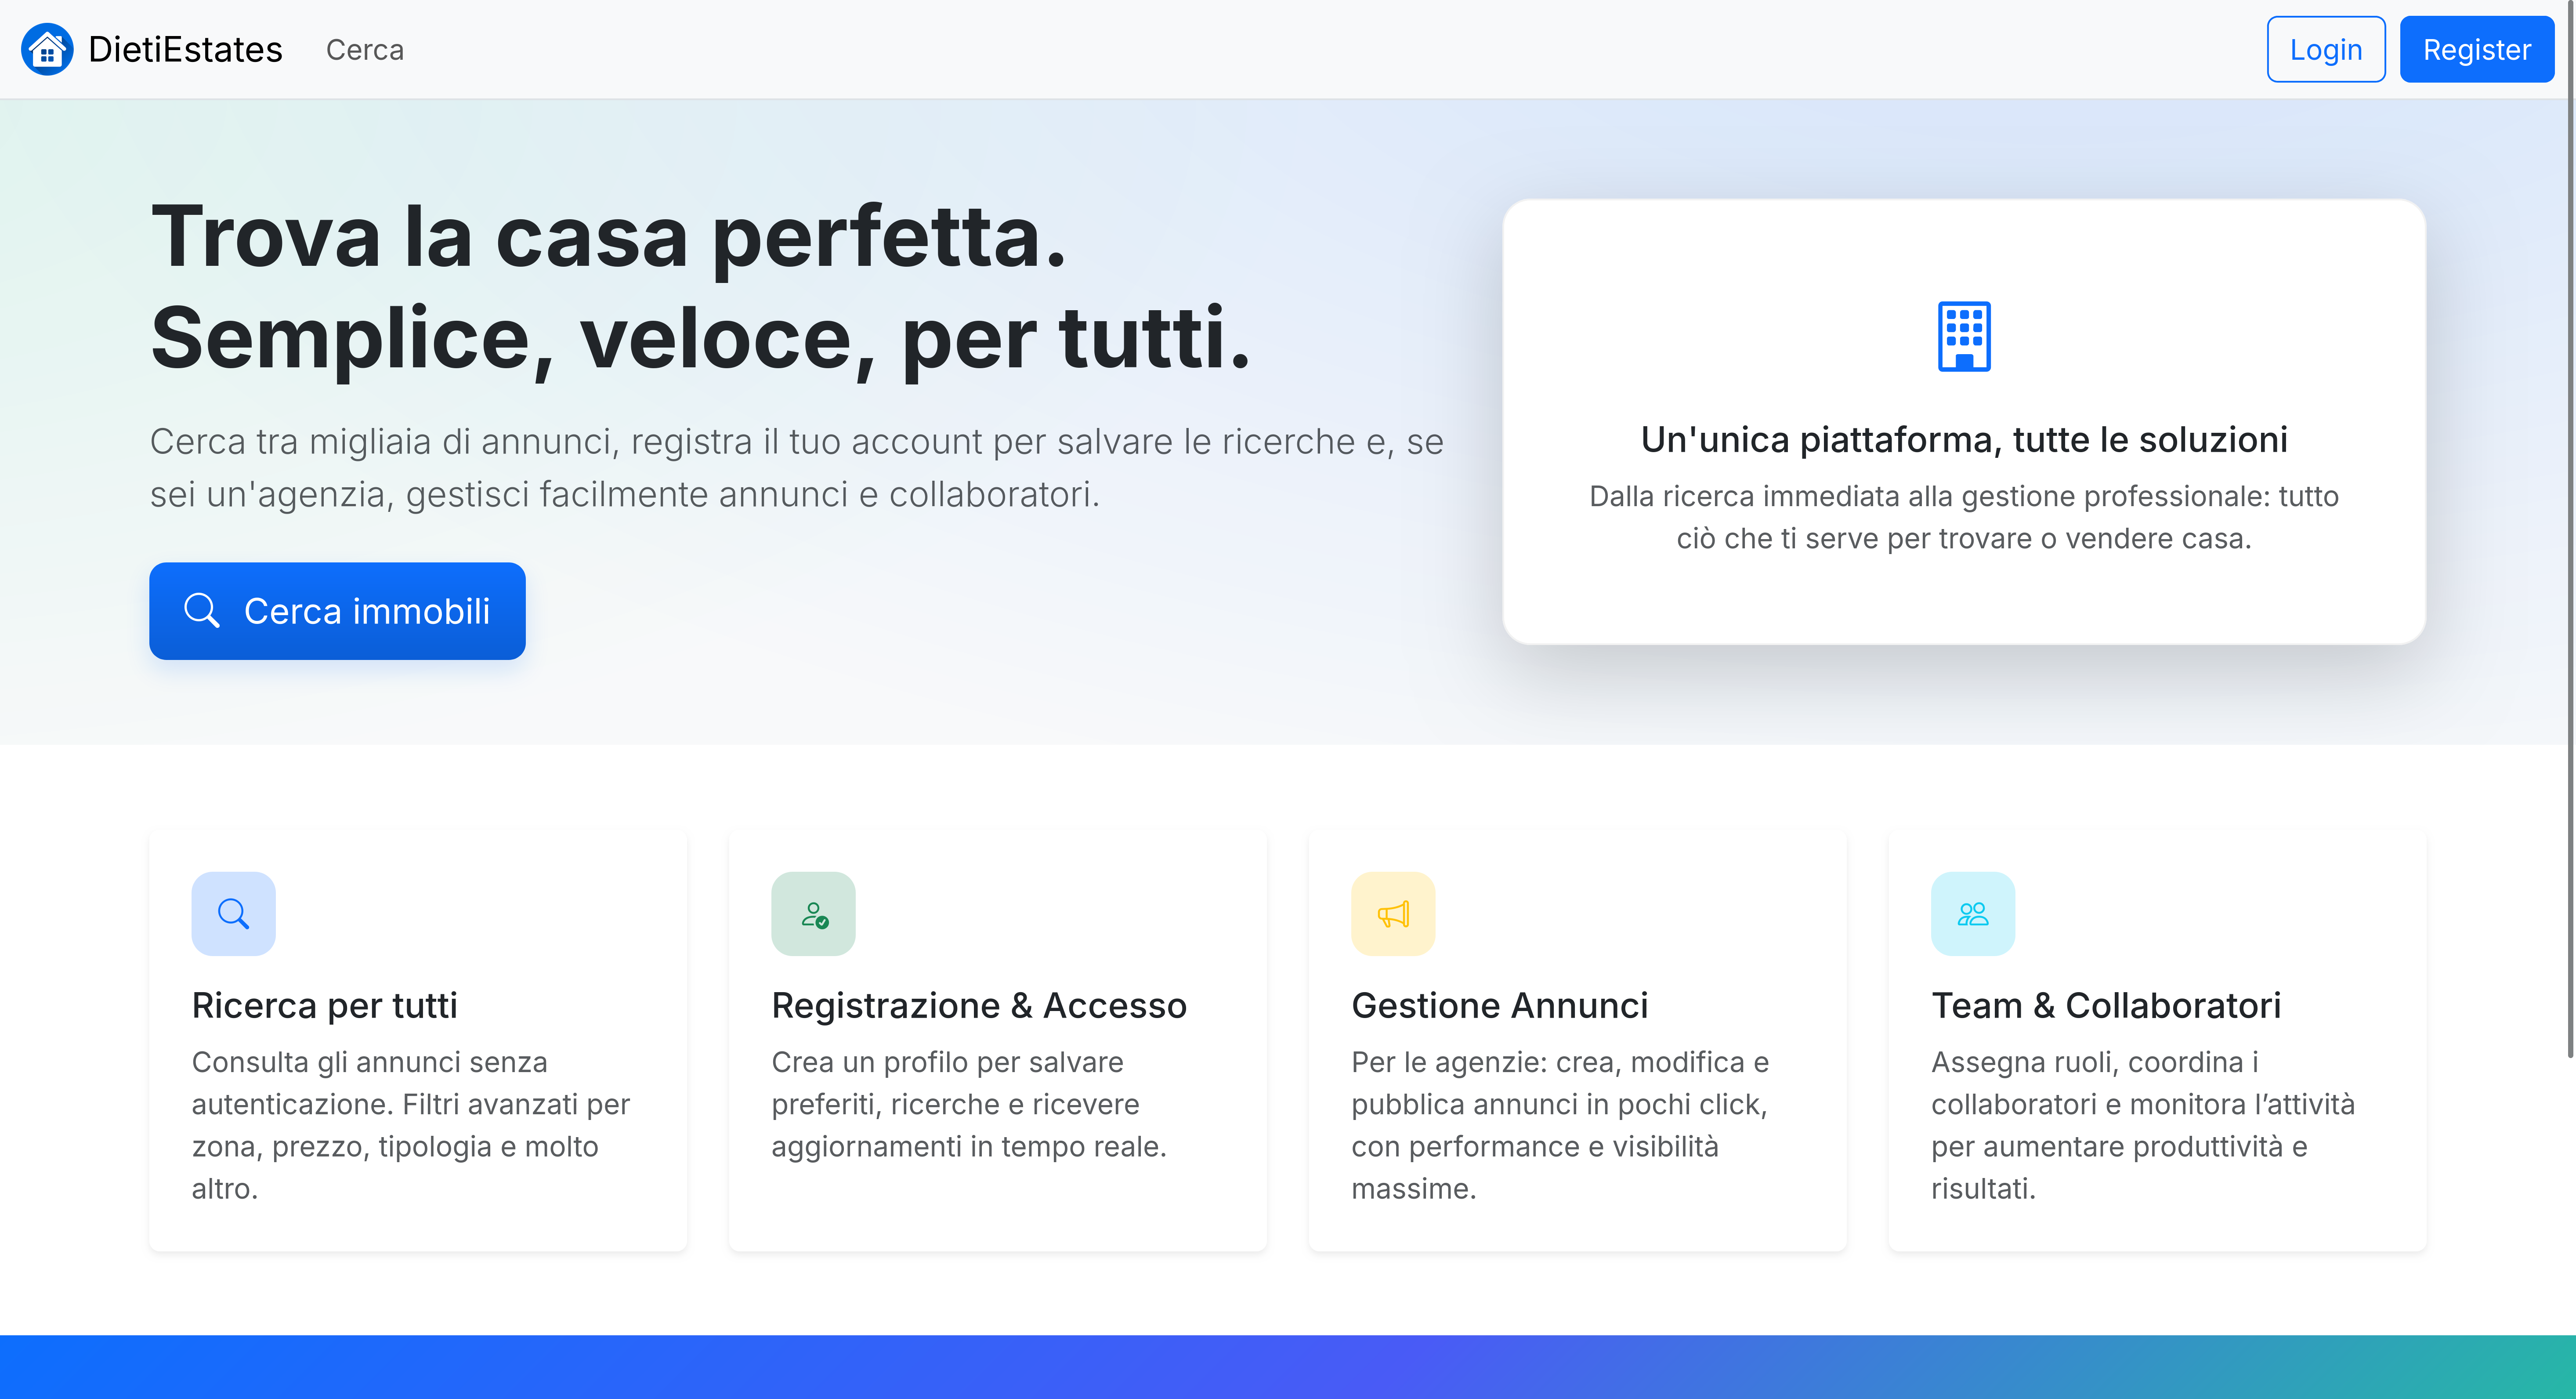
\includegraphics[width=\linewidth]{res/Mockups/homepage_unauth_user.png}
	\captionof{figure}{Homepage per un utente non autenticato}\label{fig:homepage_v1}
\end{center}

\begin{center}
	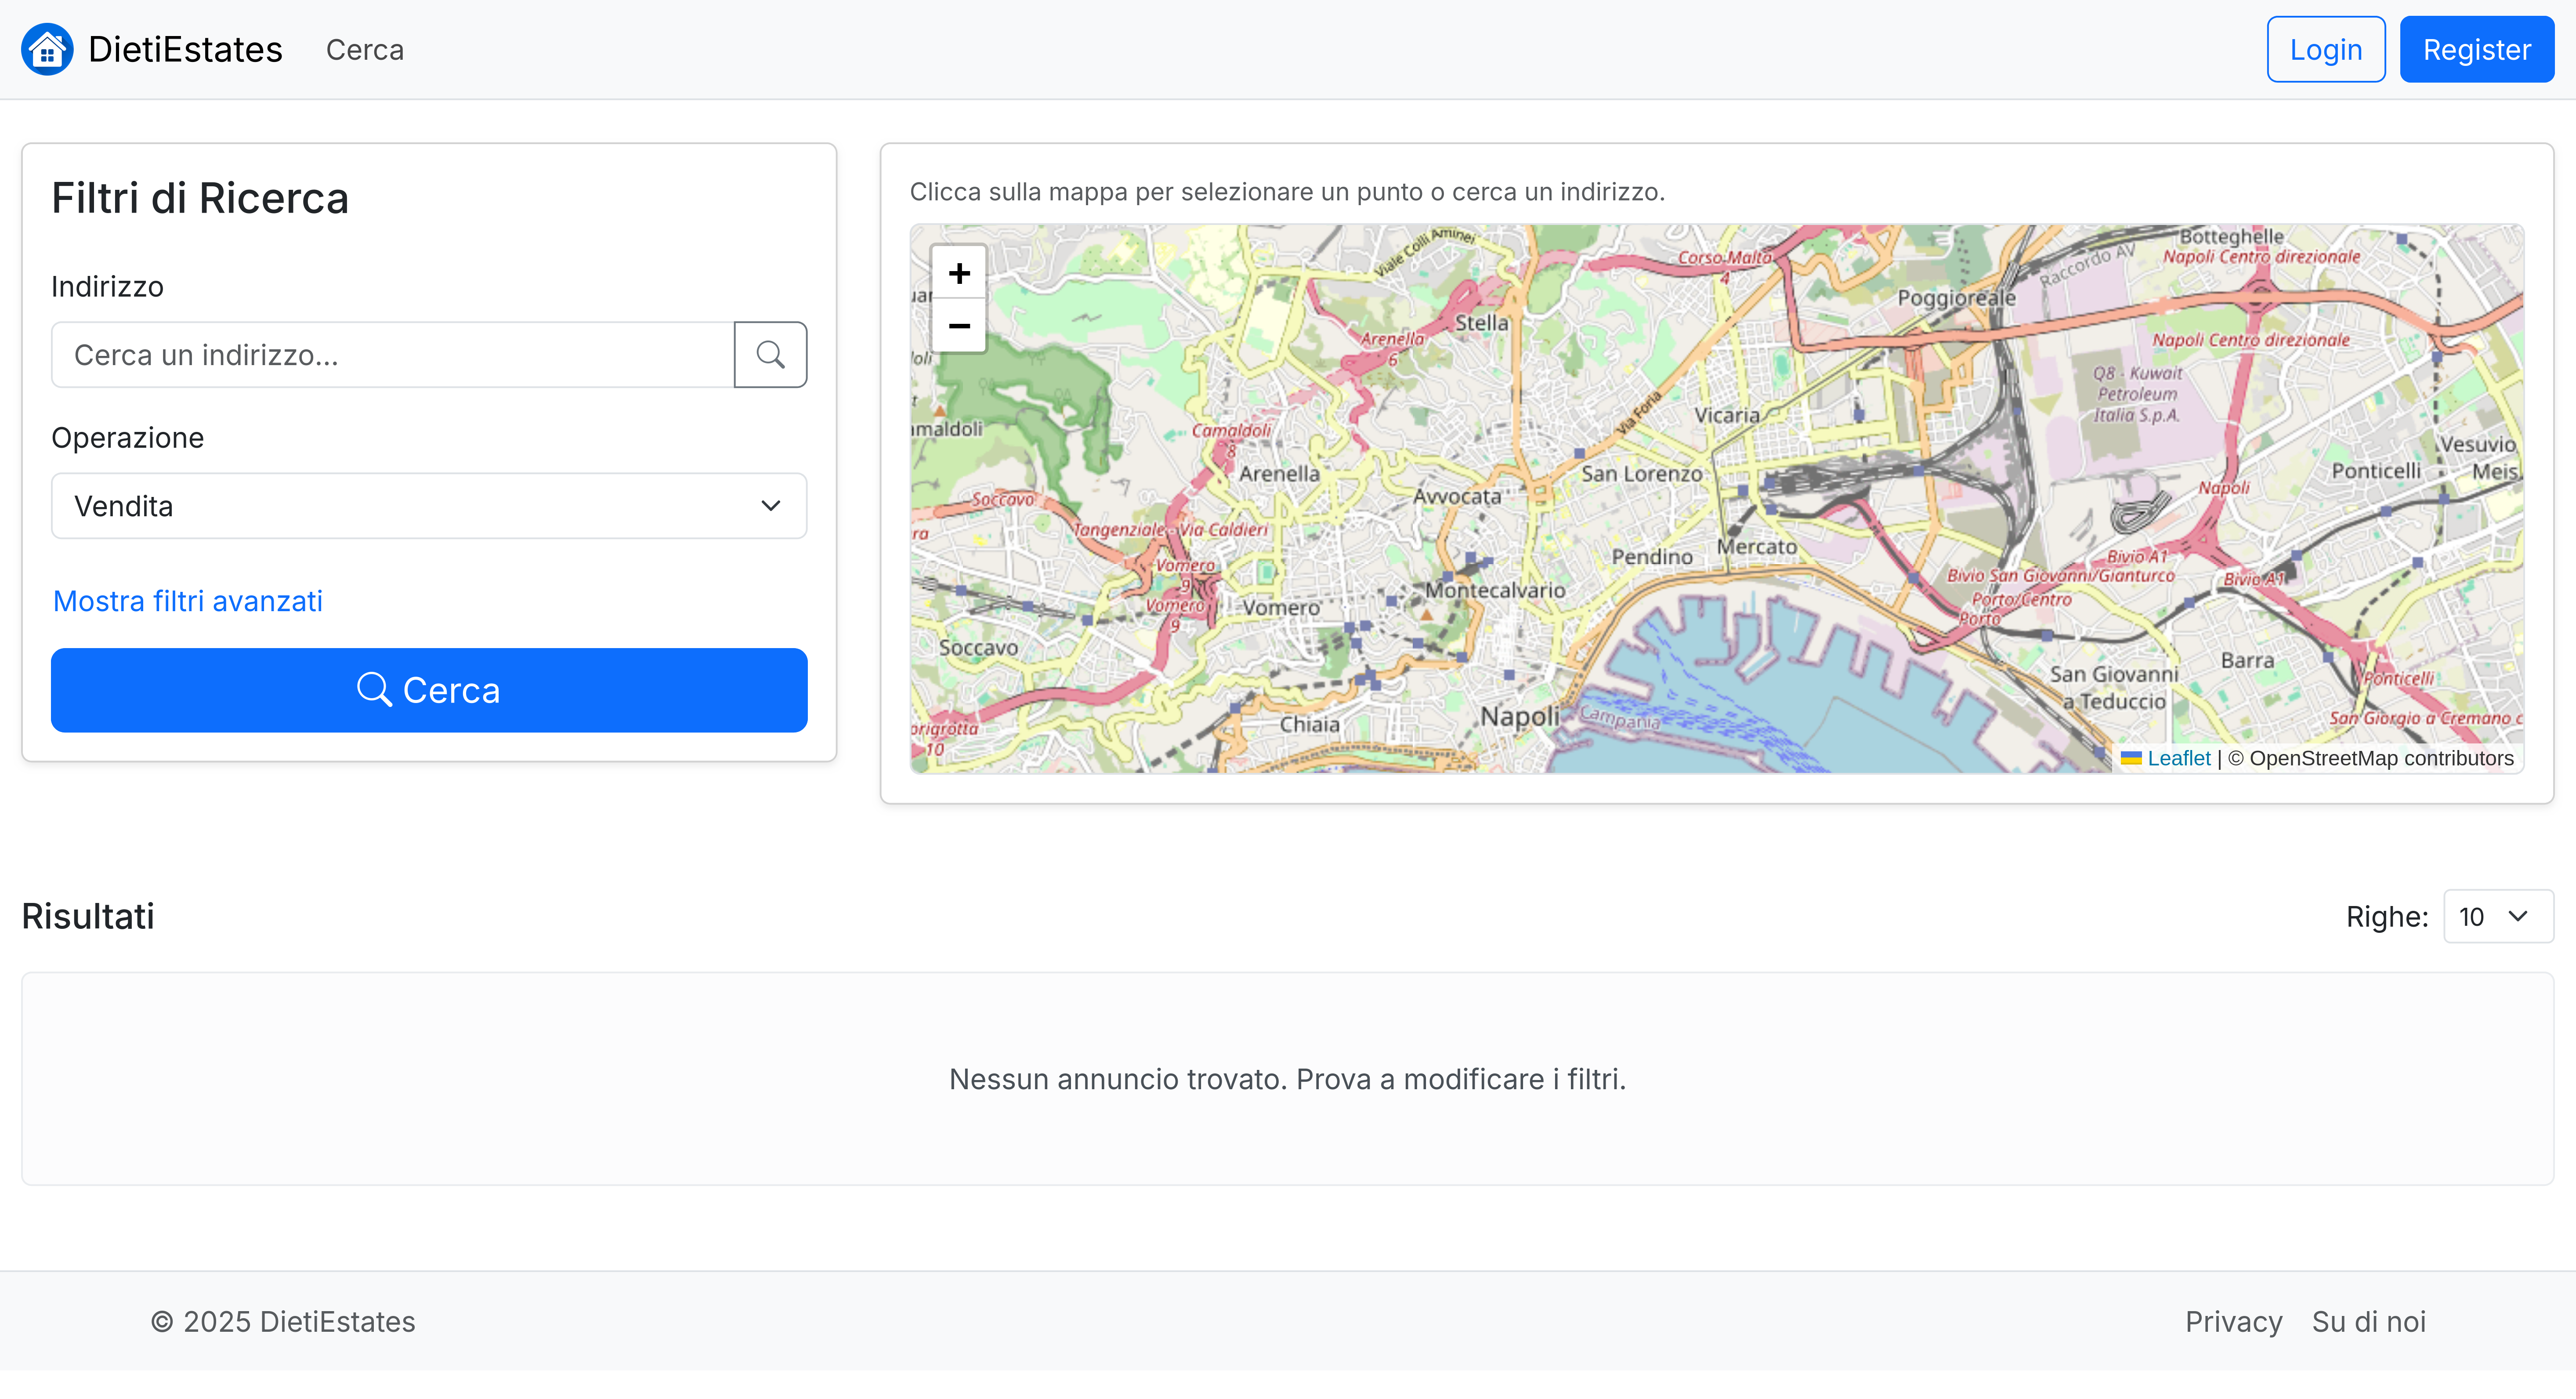
\includegraphics[width=\linewidth]{res/Mockups/normal_search_page.png}
	\captionof{figure}{Pagina per la ricerca di base}\label{fig:search_v1}
\end{center}

\begin{center}
	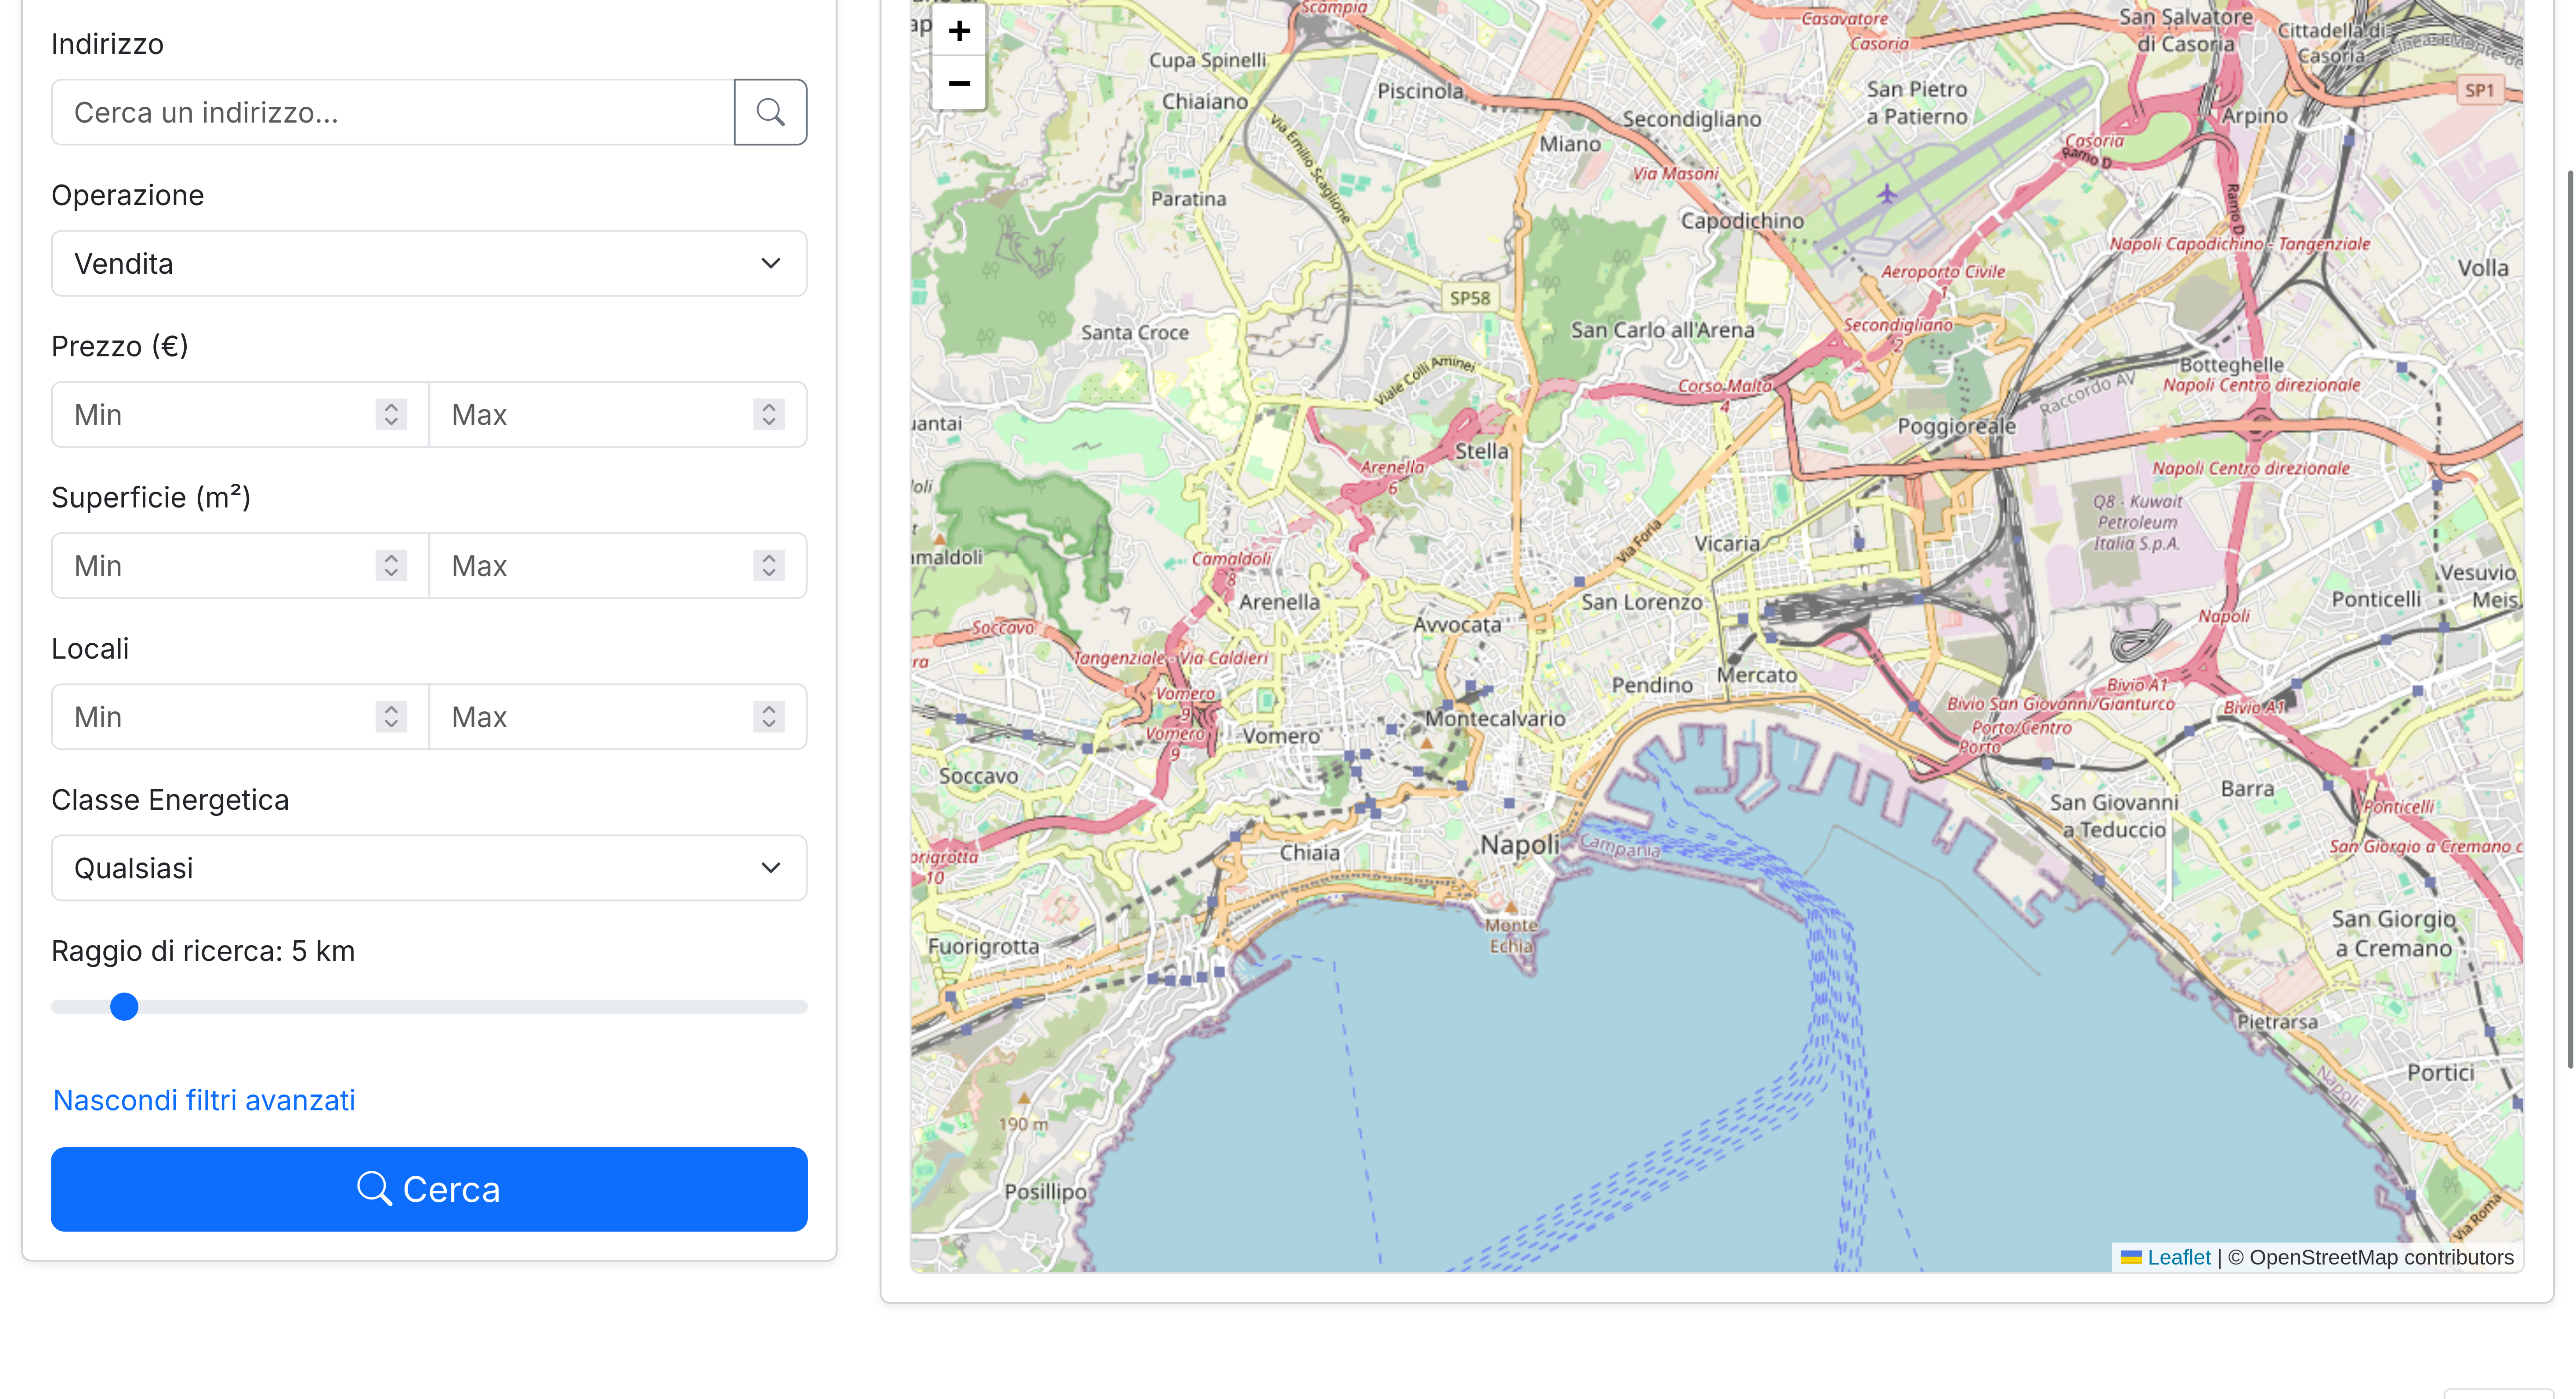
\includegraphics[width=\linewidth]{res/Mockups/advanced_search_page.png}
	\captionof{figure}{Pagina per la ricerca di base}\label{fig:search_v2}
\end{center}


\subsection{Caricamento di un annuncio immobiliare}



\begin{longtblr}
	{
		width = \linewidth,
		colspec={XXXX},
		hlines,
		vlines,
	}
	
	\textbf{Use Case \#2} & \SetCell[c=3]{l} Aggiunta annuncio immobiliare  \\
	
	\textbf{Goal in context} & \SetCell[c=3]{l} Aggiungere un nuovo annuncio \\
	
	\textbf{Precontions} & \SetCell[c=3]{l} {Un annuncio può essere creato da un agente immobiliare \\ 
		o un gestore di un'agenzia immobiliare precedentemente autenticato.}  \\
	
	\textbf{Success End Condition} & \SetCell[c=3]{l} {L’annuncio viene aggiunto al database e visibile nella pagina degli annunci listati \\ dall'agente, oltre che raggiungibile mediante la pagina di ricerca} \\
	
	\textbf{Failed End Condition} & \SetCell[c=3]{l} L’annuncio non viene inserito   \\
	
	\textbf{Primary Actor} & \SetCell[c=3]{l} Agente immobiliare o gestore di un'agenzia immobiliare  \\
	
	\textbf{Trigger} & \SetCell[c=3]{l} Viene cliccata la CTA ``Aggiungi annuncio'' dalla schermata \ref{fig:listings_management}  \\
	
	\textbf{Main Scenario} & \textbf{Step n°} & \textbf{Agente} & \textbf{Sistema} \\
	\cline{2-4} & 1 &  Clicca sulla CTA ``Aggiungi annuncio'' nella  schermata \ref{fig:listings_management} &  \\
	\cline{2-4} & 2 & & Apre schermata \ref{fig:listings_form} \\
	\cline{2-4} & 3 & Aggiunge titolo dell'annuncio & \\
	\cline{2-4} & 4 & Aggiunge descrizione dell'annuncio & \\
	\cline{2-4} & 5 & Aggiunge tipologia dell'annuncio, se vendita oppure affitto & \\
	\cline{2-4} & 6 & Aggiunge prezzo dell'annuncio & \\
	\cline{2-4} & 7 & Aggiunge immagini dell'immobile & \\
	\cline{2-4} & 8 & Inserisce indirizzo e preme ``Cerca'' & \\
	\cline{2-4} & 9 & & Chiama servizio esterno Nominatim per prelevare coordinate dell'indirizzo \\
	\cline{2-4} & 10 & & Mostra marker sulla mappa interattiva per indicare la posizione dell'immobile\\
	\cline{2-4} & 11 & Preme ``Salva'' & \\
	\cline{2-4} & 12 & & Valida il form. \\
	\cline{2-4} & 13 & & Salva l'annuncio nel database. \\
	\cline{2-4} & 14 & & Reindirizza l'utente alla pagina \ref{fig:listings_management} mostrando una nuova card per l'annuncio appena creato. Fine del caso d'uso. \\
	\textbf{Extension \#1: Utente preme ``Salva'' senza aver caricato una foto} & \textbf{Step n°} & \textbf{Agente} & \textbf{Sistema} \\
	\cline{2-4} & 1.13 & & Mostra messaggio di errore ``Caricare almeno un'immagine'' \\
	\textbf{Extension \#2: Utente preme salva senza aver compilato campi obbligatori} & \textbf{Step n°} & \textbf{Agente} & \textbf{Sistema} \\
	\cline{2-4} & 2.12 & & Mostra messaggio di errore ``Compila campi obbligatori'' \\
	\textbf{Extension \#3: Utente preme ``Annulla''} & \textbf{Step n°} & \textbf{Agente} & \textbf{Sistema} \\
	\cline{2-4} & 3.2 & & Mostra messaggio di conferma \\
	\cline{2-4} & 3.3 & Preme ``Conferma'' & \\
	\cline{2-4} & 3.4 & & Reindirizza l'utente alla pagina \ref{fig:listings_management} senza aggiungere l'annuncio. \\
\end{longtblr}


\begin{center}
	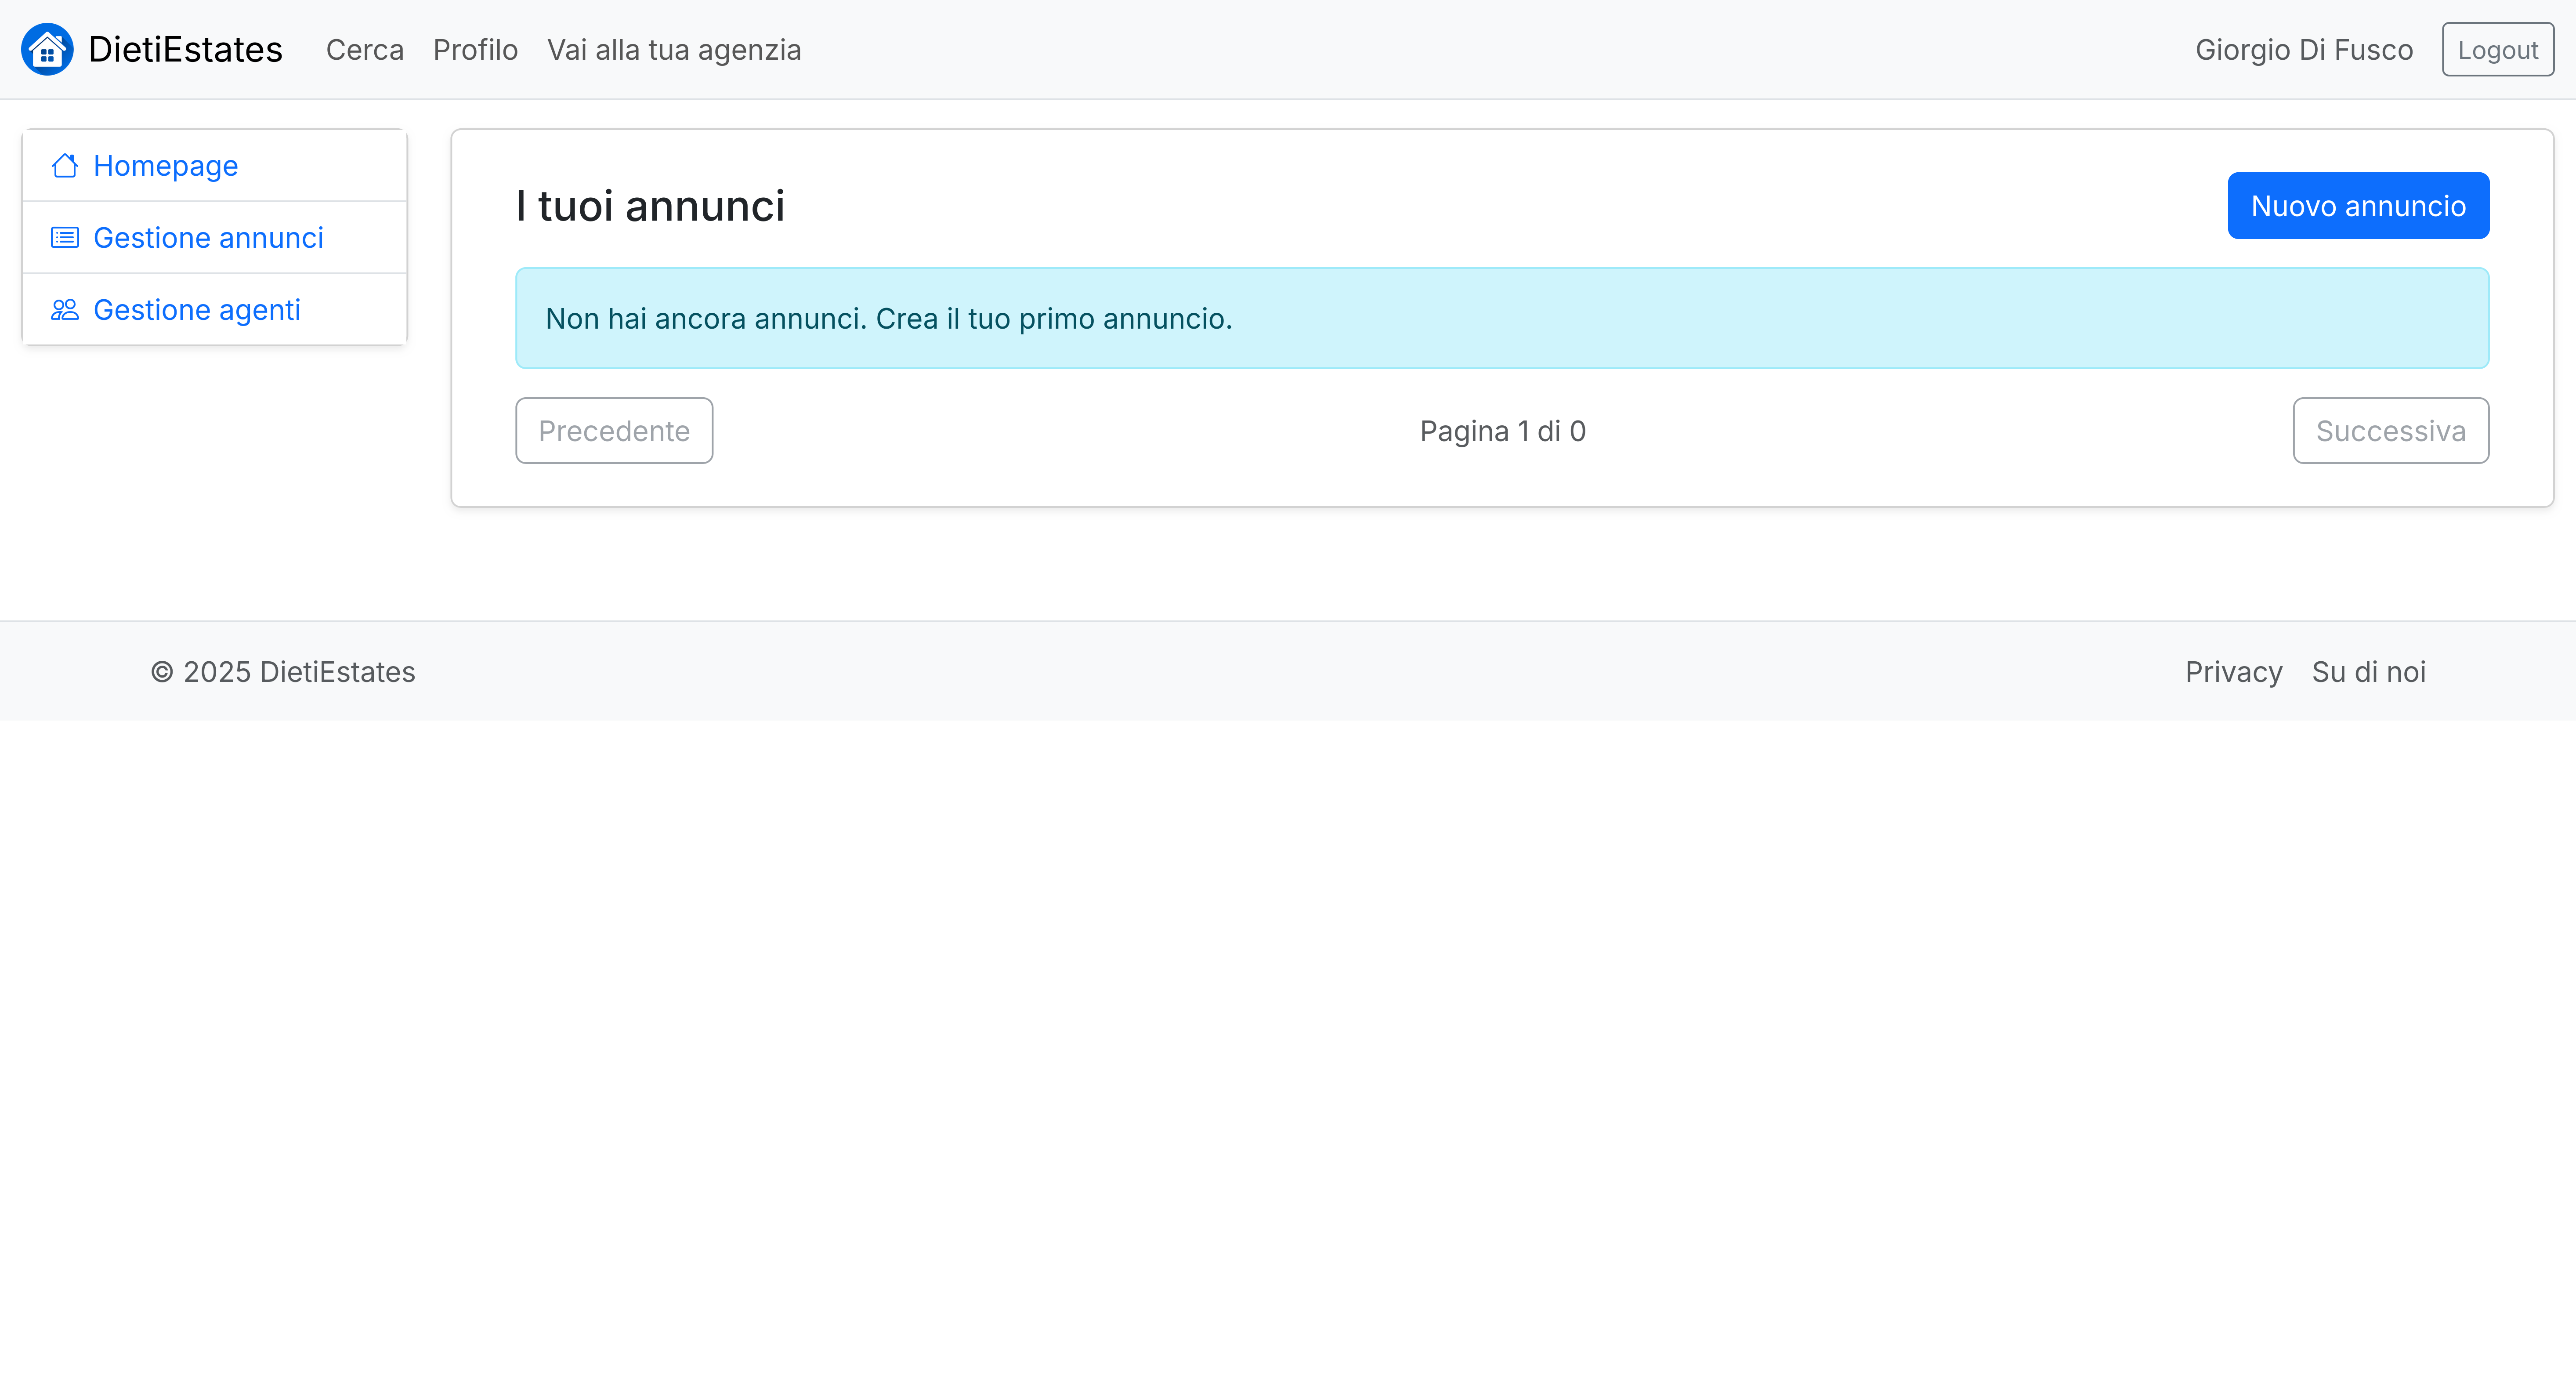
\includegraphics[width=\linewidth]{res/Mockups/addlistinghomepage.png}
	\captionof{figure}{Pagina per la gestione degli annunci immobiliari}\label{fig:listings_management}
\end{center}


\begin{center}
	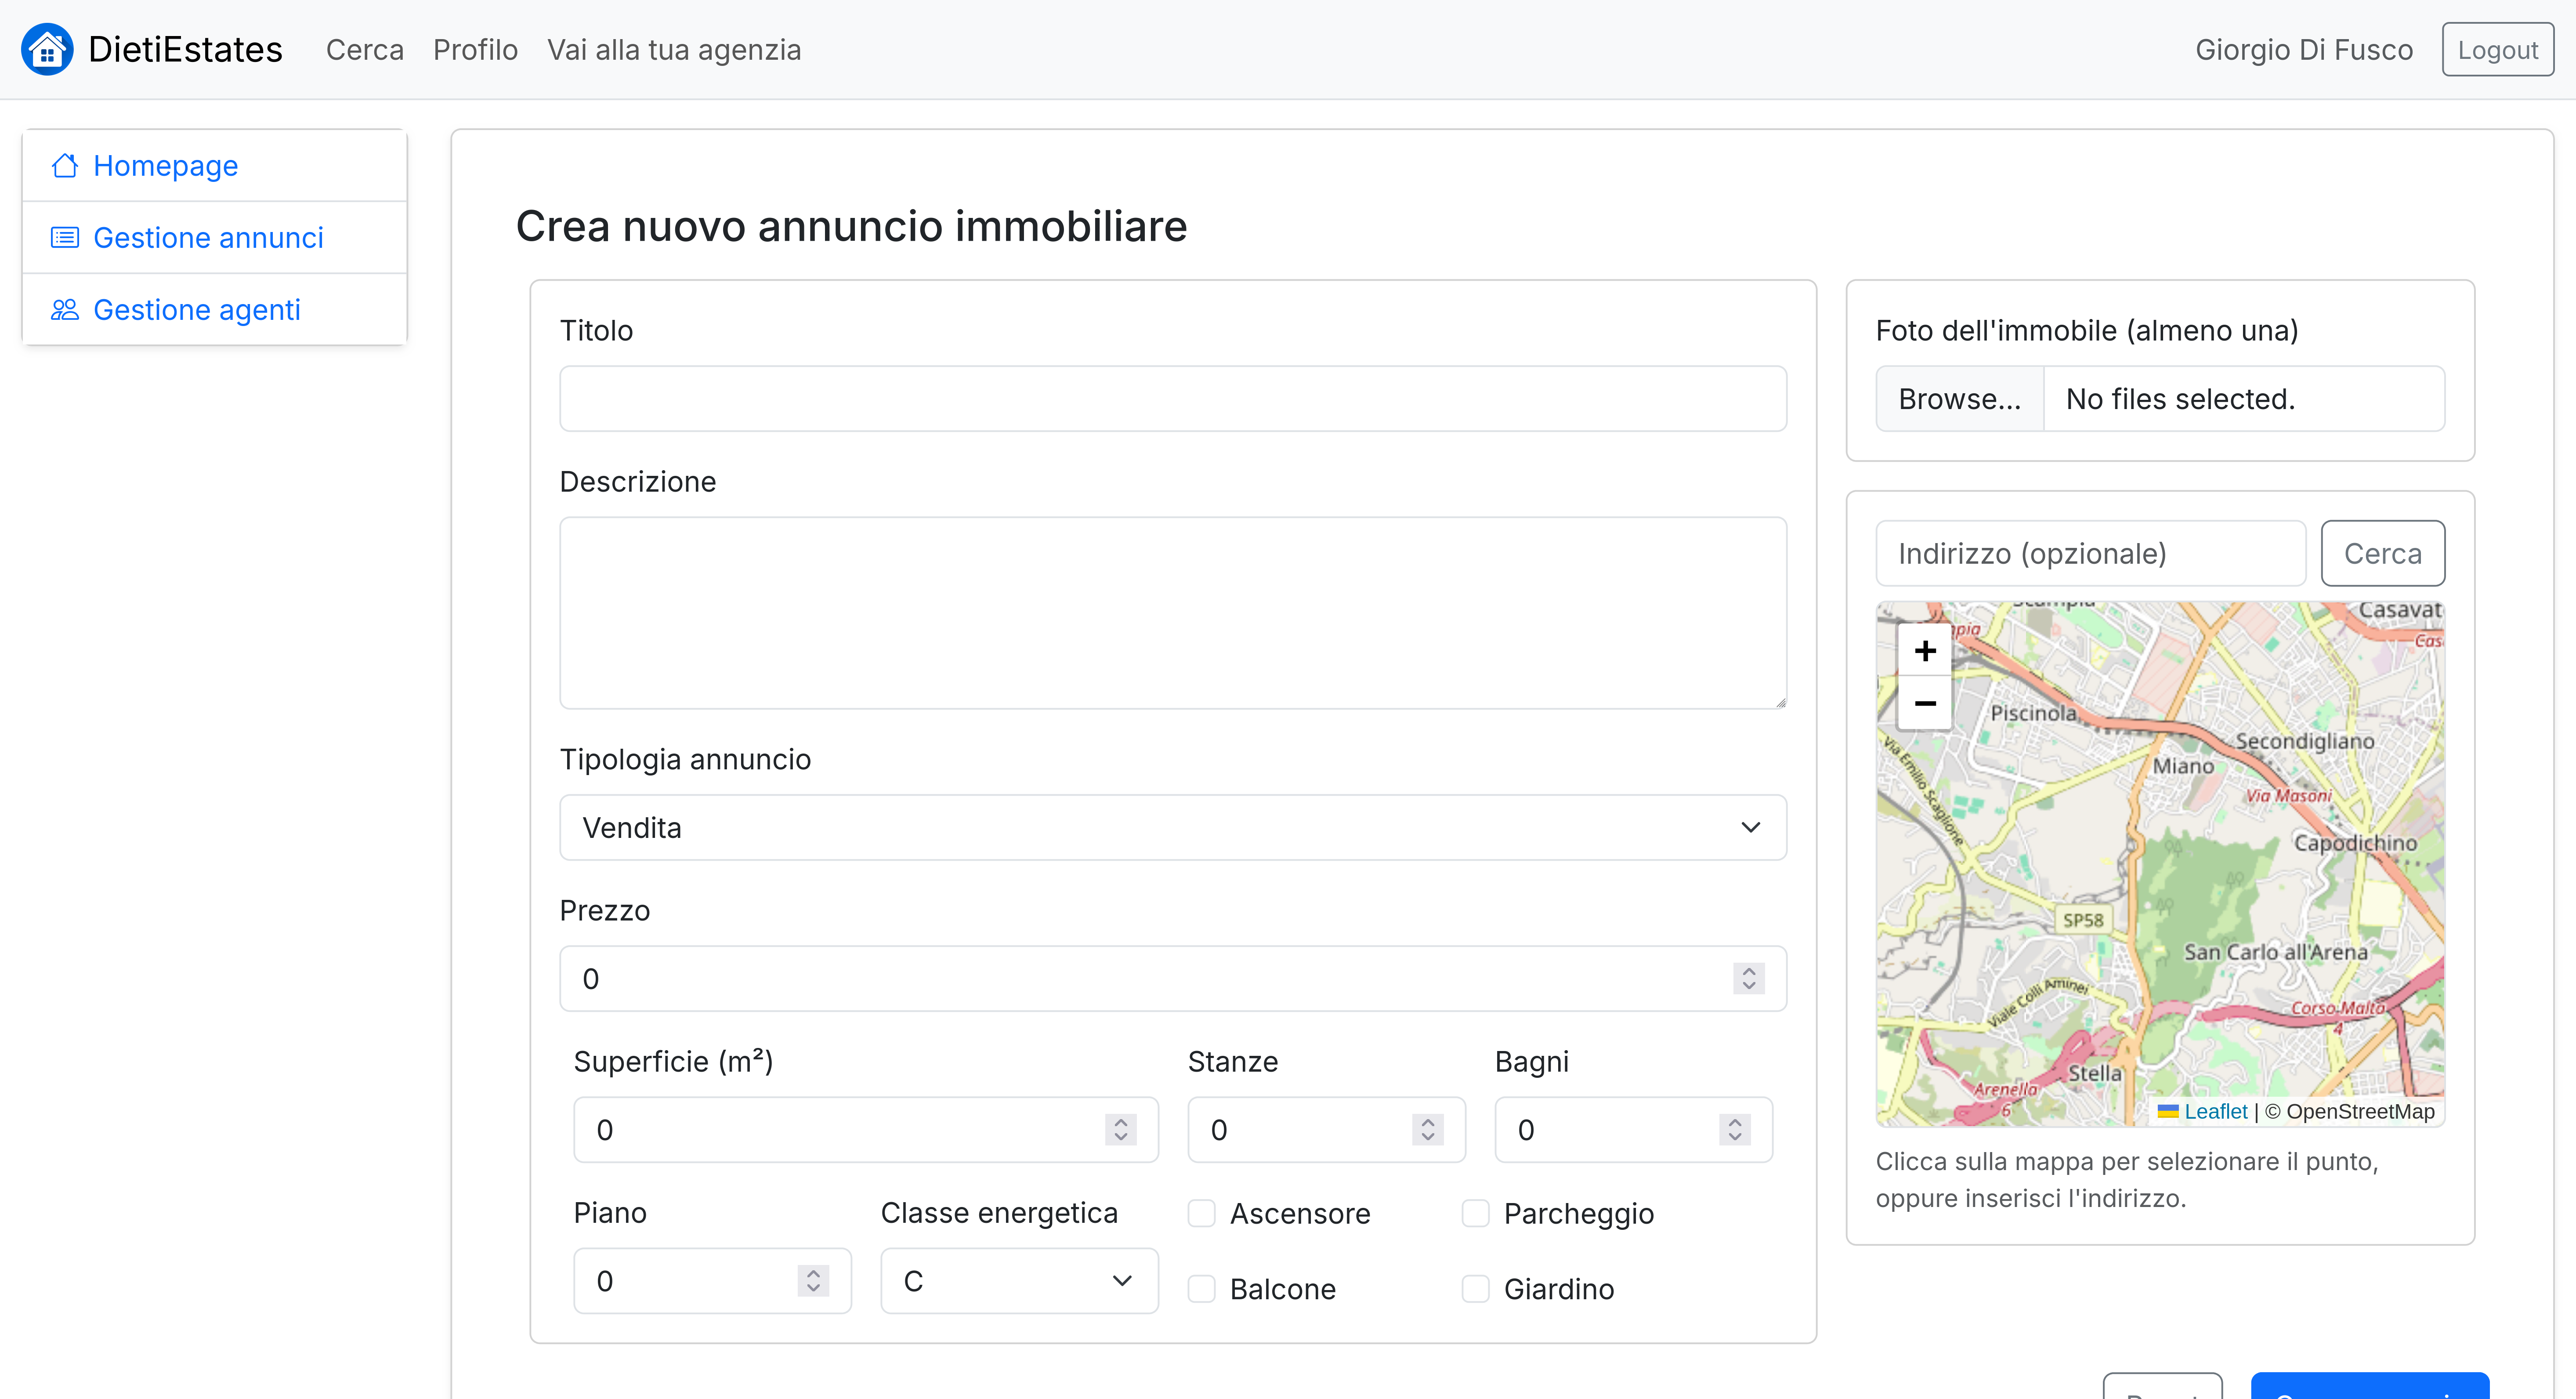
\includegraphics[width=\linewidth]{res/Mockups/addlistingform.png}
	\captionof{figure}{Pagina per l'aggiunta per un nuovo annuncio immobiliare}\label{fig:listings_form}
\end{center}


\begin{center}
	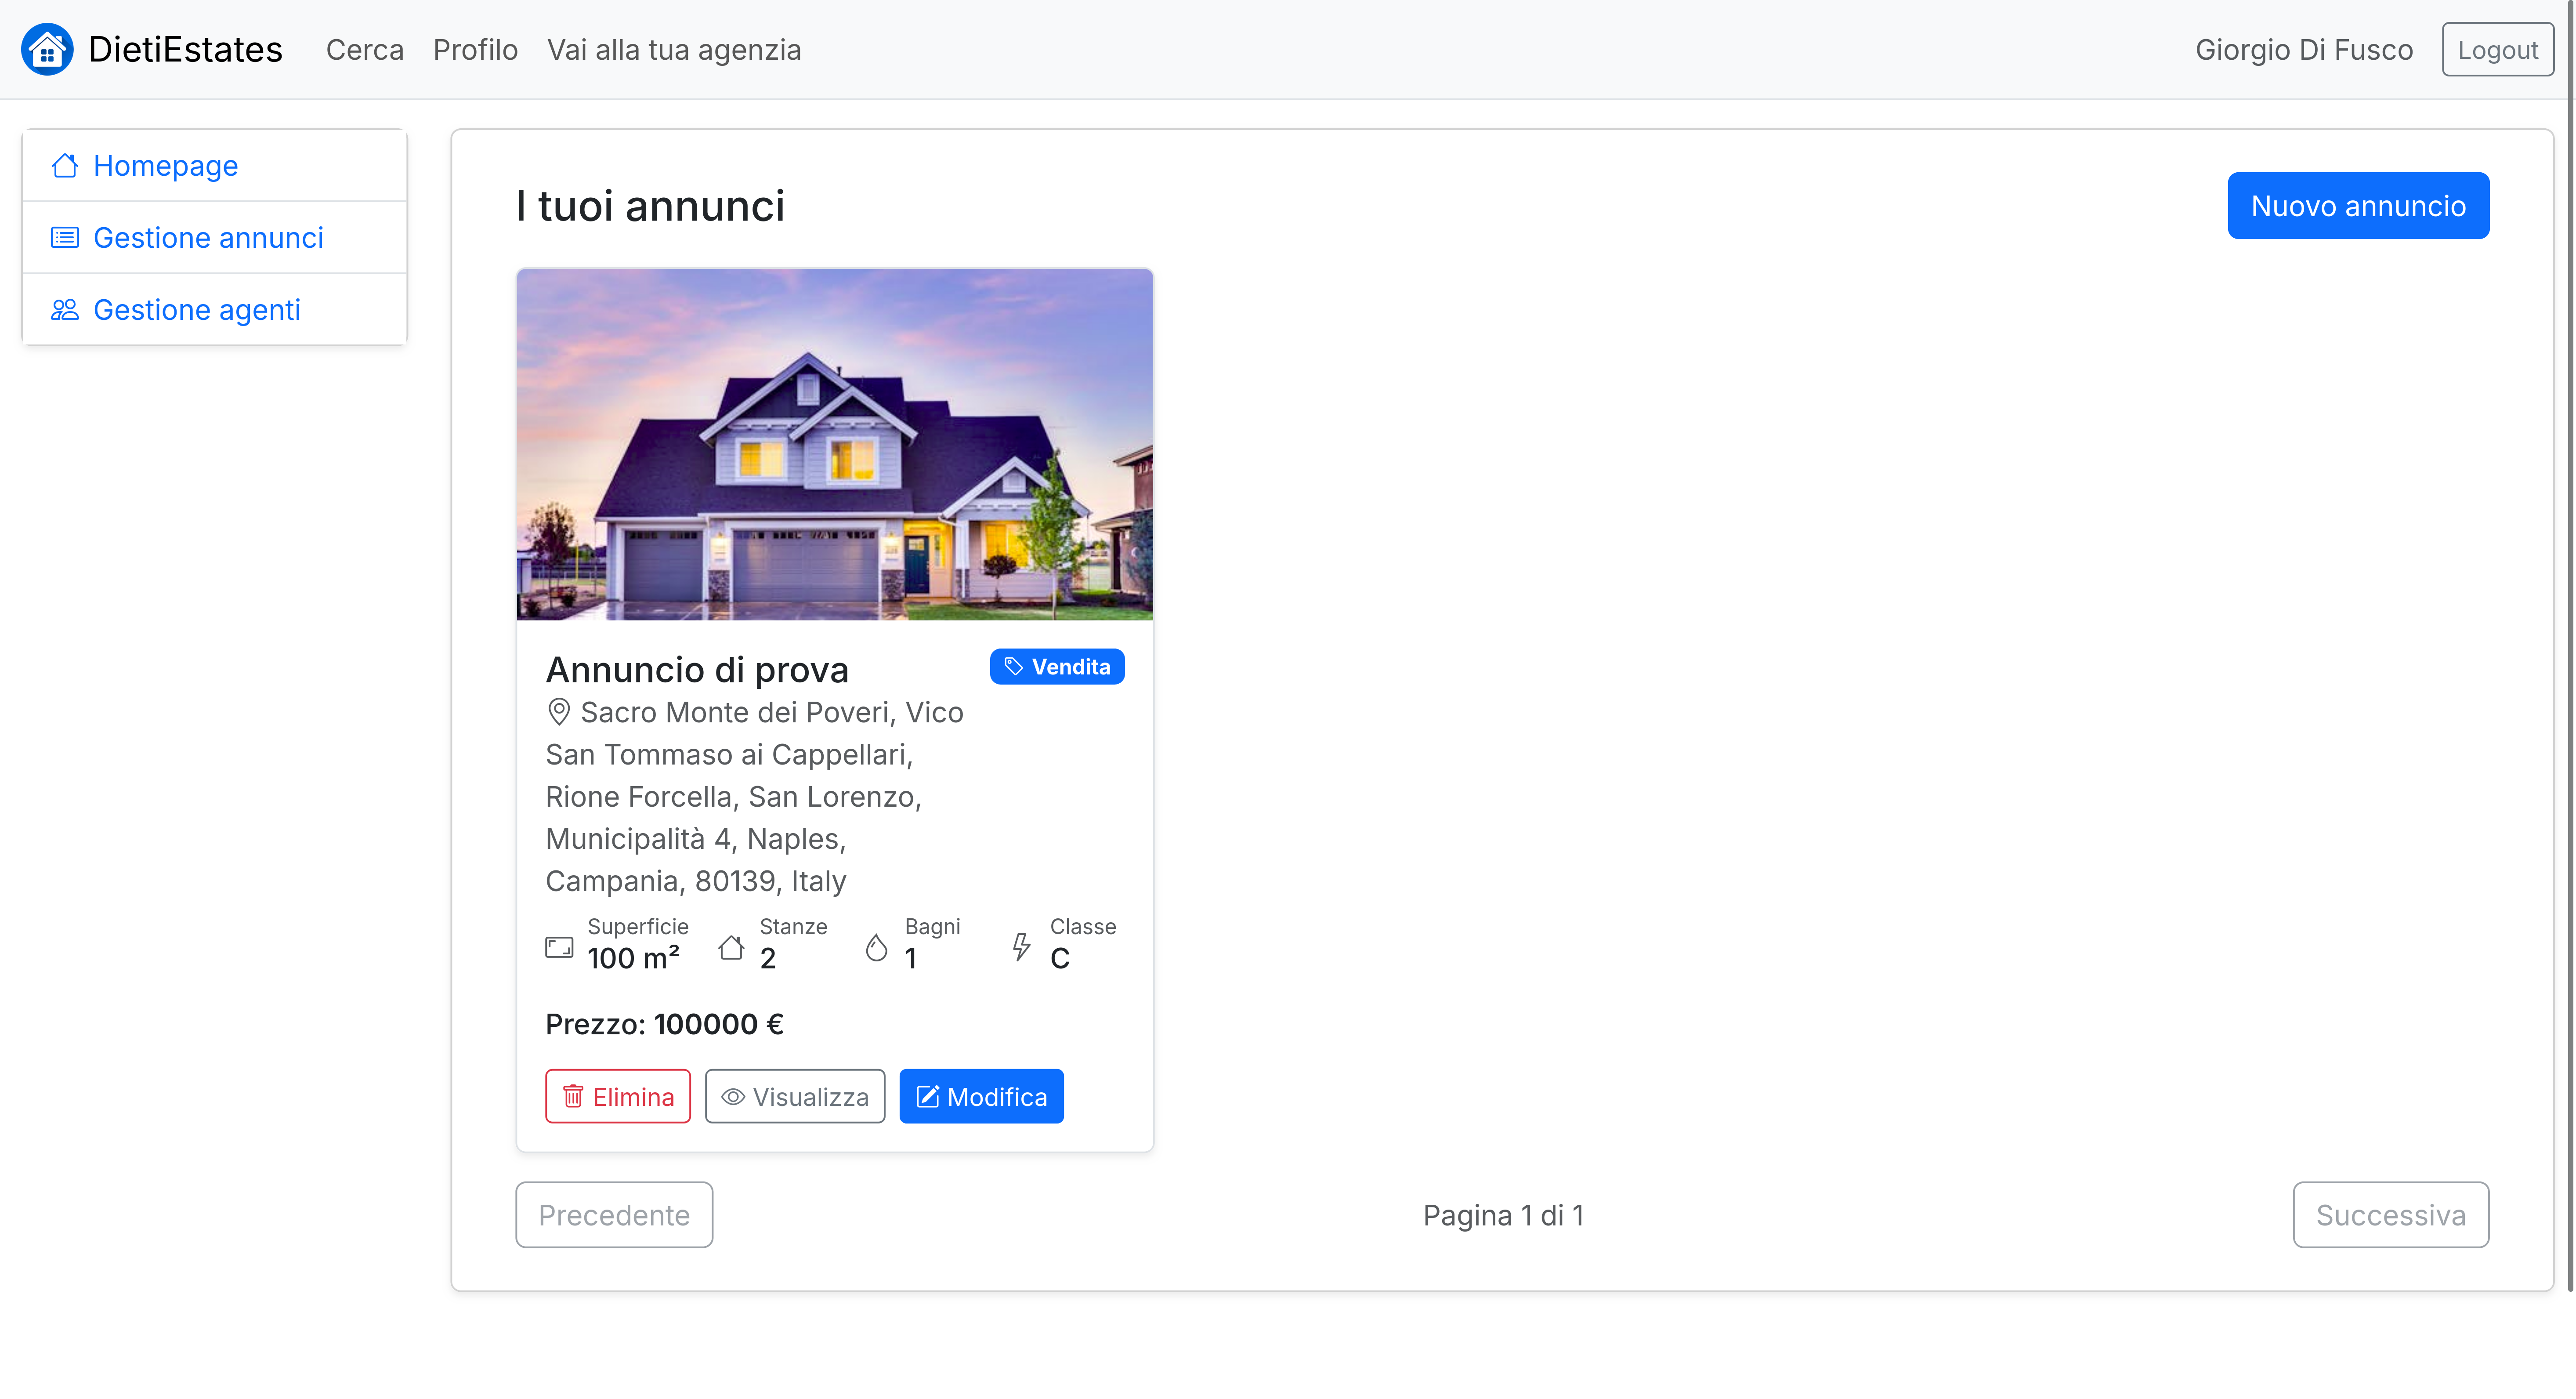
\includegraphics[width=\linewidth]{res/Mockups/listing_management_populated.png}
	\captionof{figure}{Pagina con la card aggiornata}\label{fig:listings_management_with_card}
\end{center}
\subsection{Aggiunta di un agente immobiliare}
\begin{longtblr}{
		width = \linewidth,
		colspec={XXXX},
		hlines,
		vlines,
	}
	\textbf{Use Case \#3} & \SetCell[c=3]{l} Aggiunta di un nuovo agente immobiliare \\
	
	\textbf{Goal in Context} & \SetCell[c=3]{l} Il gestore di un'agenzia immobiliare vuole aggiungere un nuovo agente \\
	
	\textbf{Preconditions} & \SetCell[c=3]{l}  L’utente possiede ruolo \texttt{ROLE\_ADMIN} oppure \texttt{ROLE\_ADMIN\_ASSISTANT} \\
	
	\textbf{Success End Condition} & \SetCell[c=3]{l} Il collaboratore viene associato all'agenzia \\
	
	\textbf{Failed End Condition} & \SetCell[c=3]{l} Non viene inserita l'associazione utente-agenzia. \\
	
	\textbf{Primary Actor} & \SetCell[c=3]{l} Gestore di una agenzia immobiliare  \\
	
	\textbf{Trigger} & \SetCell[c=3]{l} L'amministratore, dalla schermata \ref{fig:dashboard_admin}, clicca su ``Aggiungi collaboratore'' \\
	
	\textbf{Main Scenario} & \textbf{Step n°} & \textbf{Agente} & \textbf{Sistema} \\
	
	\cline{2-4} & 1 & Clicca su ``Aggiungi collaboratore'' &  \\
	
	\cline{2-4} & 2 & & Carica schermata \ref{fig:add_agent}  \\
	
	\cline{2-4} & 3 & Inserisce nome, cognome ed email dell'agente che intende inserire. &  \\
	
	\cline{2-4} & 4 & Preme su ``Salva''  & \\
	
	\cline{2-4} & 5 & & Valida i campi \\
	
	\cline{2-4} & 6 & & Mostra messaggio di successo\\
	
	\cline{2-4} & 7 & & Reindirizza l'utente alla schermata \ref{fig:dashboard_admin} \\
	
	\cline{2-4} & 8 & & {Il sistema aggiunge un account relativo all'agente con gli opportuni permessi nel database e con una password predefinita. Collega l'agente all'agenzia immobiliare }\\

	\cline{2-4} & 9 & & Invia una email all'agente con un codice di attivazione e l'invito a modificare la propria password  \\
	
	\textbf{Extension \#1: Email agente già presente} & \textbf{Step n°} & \textbf{Agente} & \textbf{Sistema} \\
	
	\cline{2-4} & 1.5 & & Il sistema individua l'utente associato alla email inserita \\
	
	\cline{2-4} & 1.6 & & Assegna ruolo \texttt{ROLE\_AGENT} all'utente e lo associa all'agenzia dell'utente che lo ha inserito \\
	
	\cline{2-4} & 1.7 & & Invia una email all'utente promosso al ruolo di agente per comunicare la promozione\\
\end{longtblr}

\begin{center}
	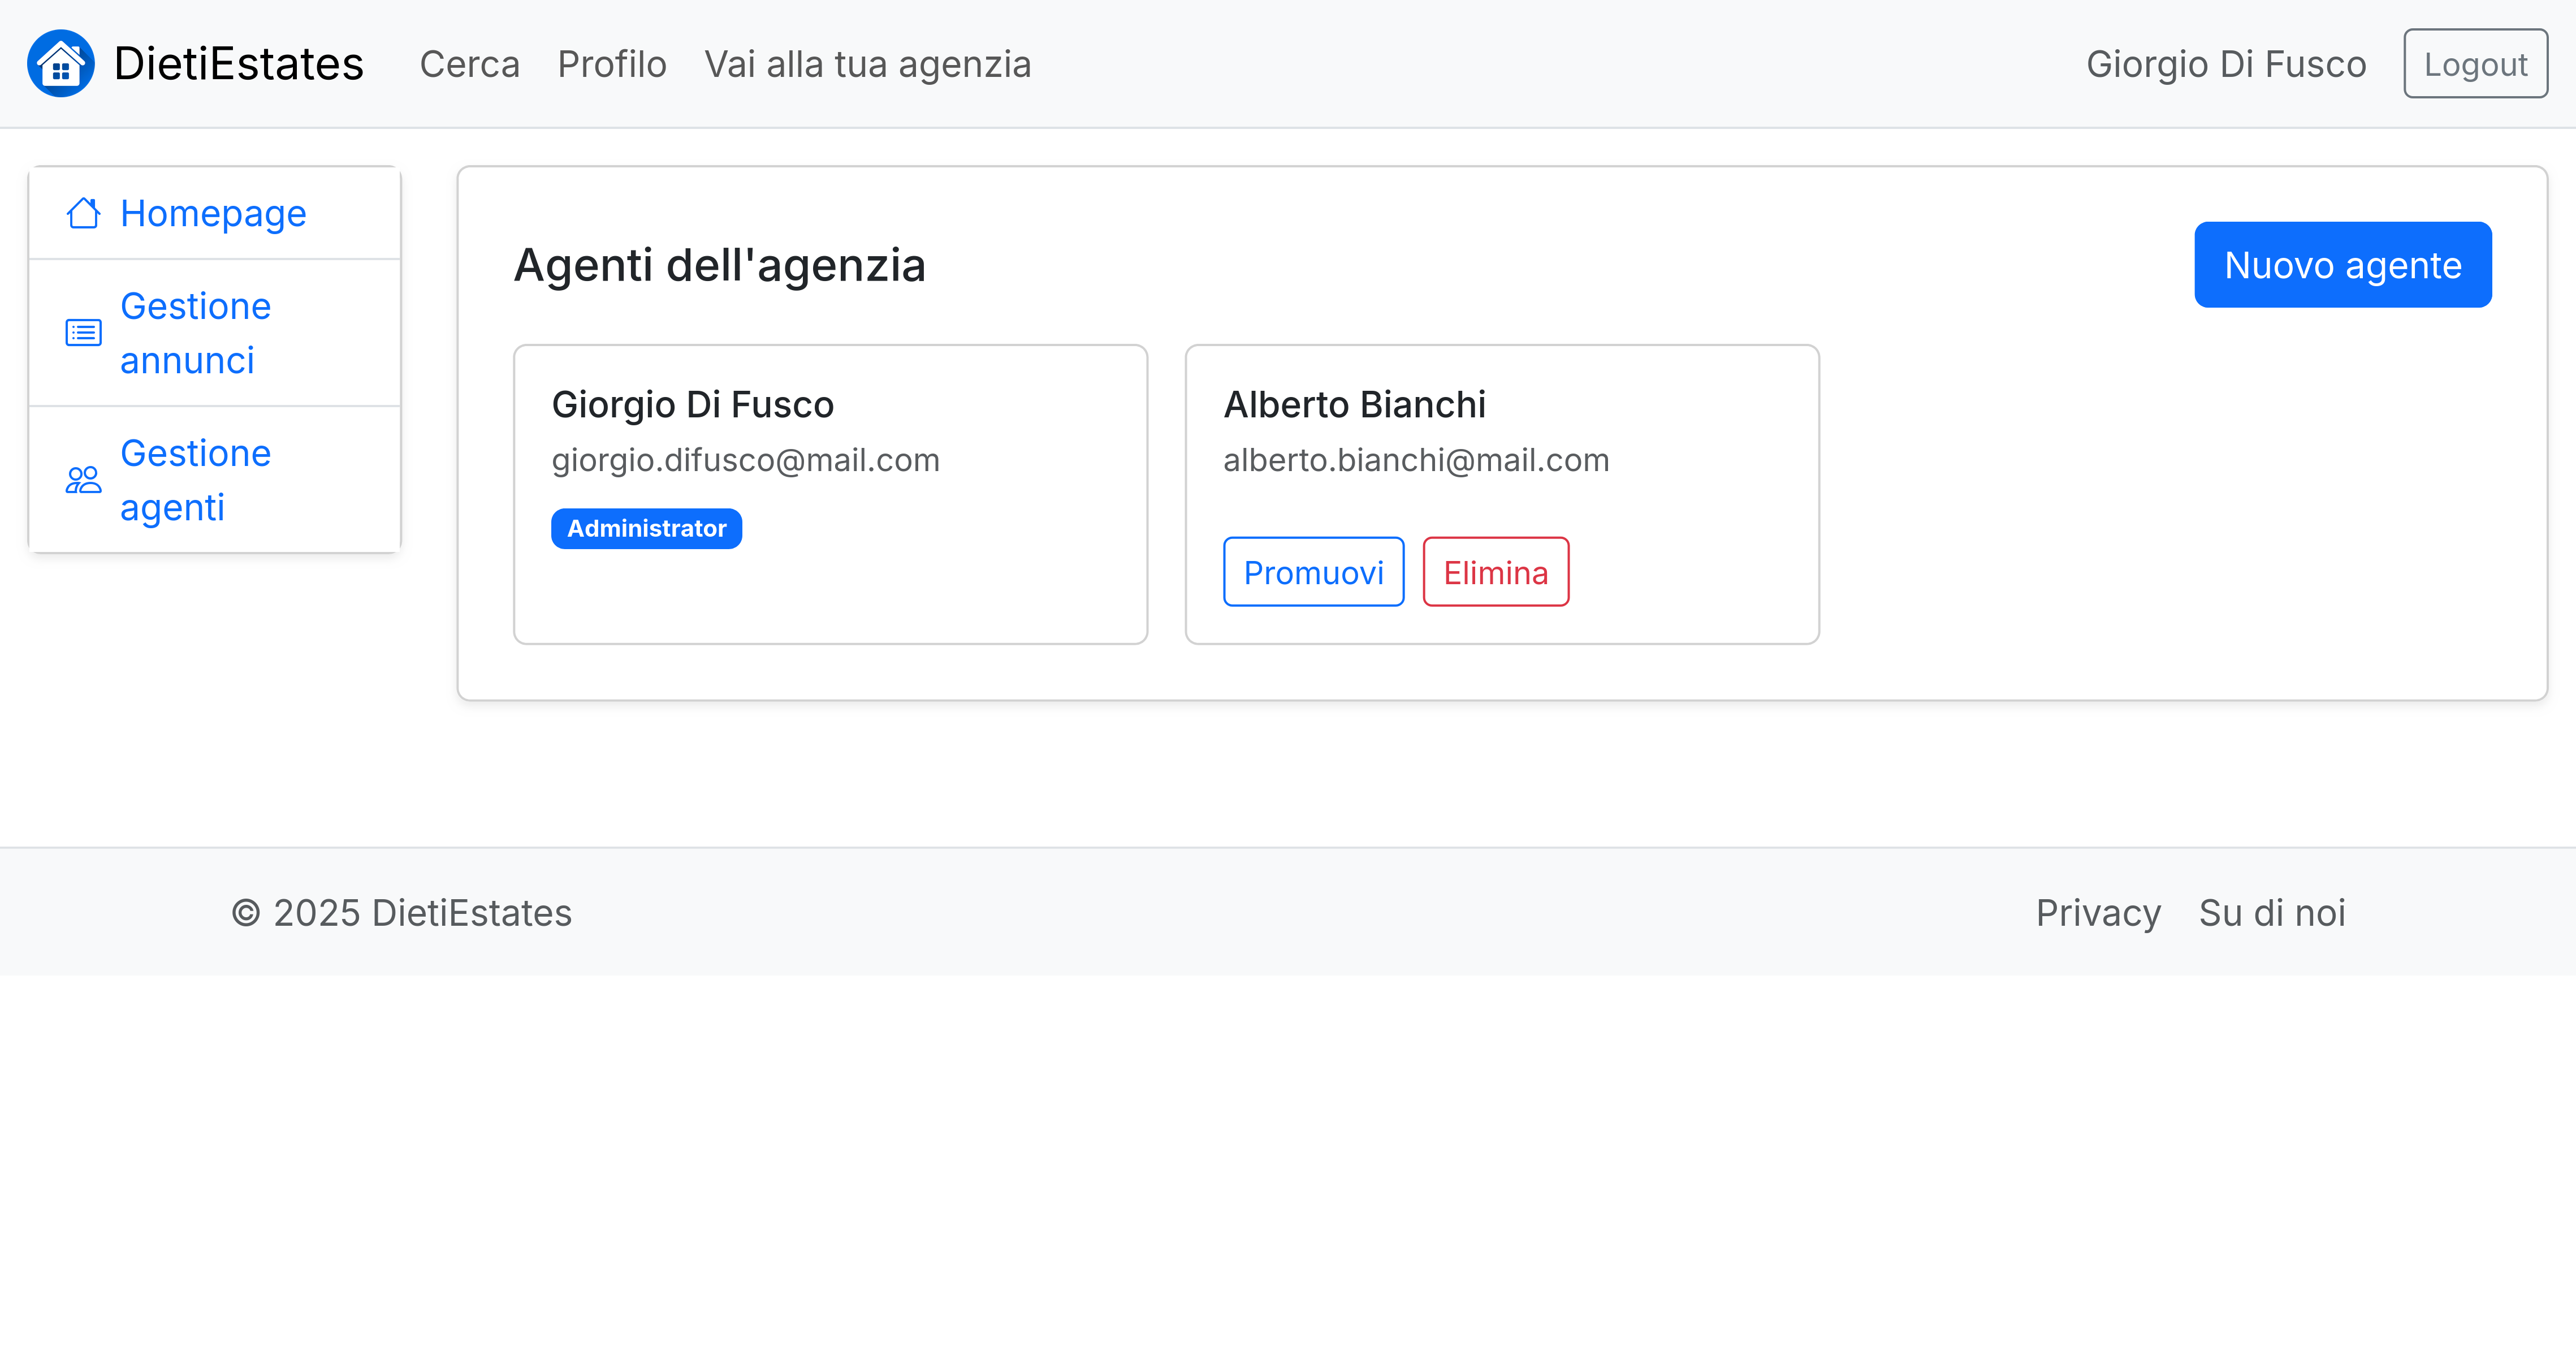
\includegraphics[width=\linewidth]{res/Mockups/agents_management.png}
	\captionof{figure}{Dashboard gestione agenti immobiliari}\label{fig:dashboard_admin}
\end{center}

\begin{center}
	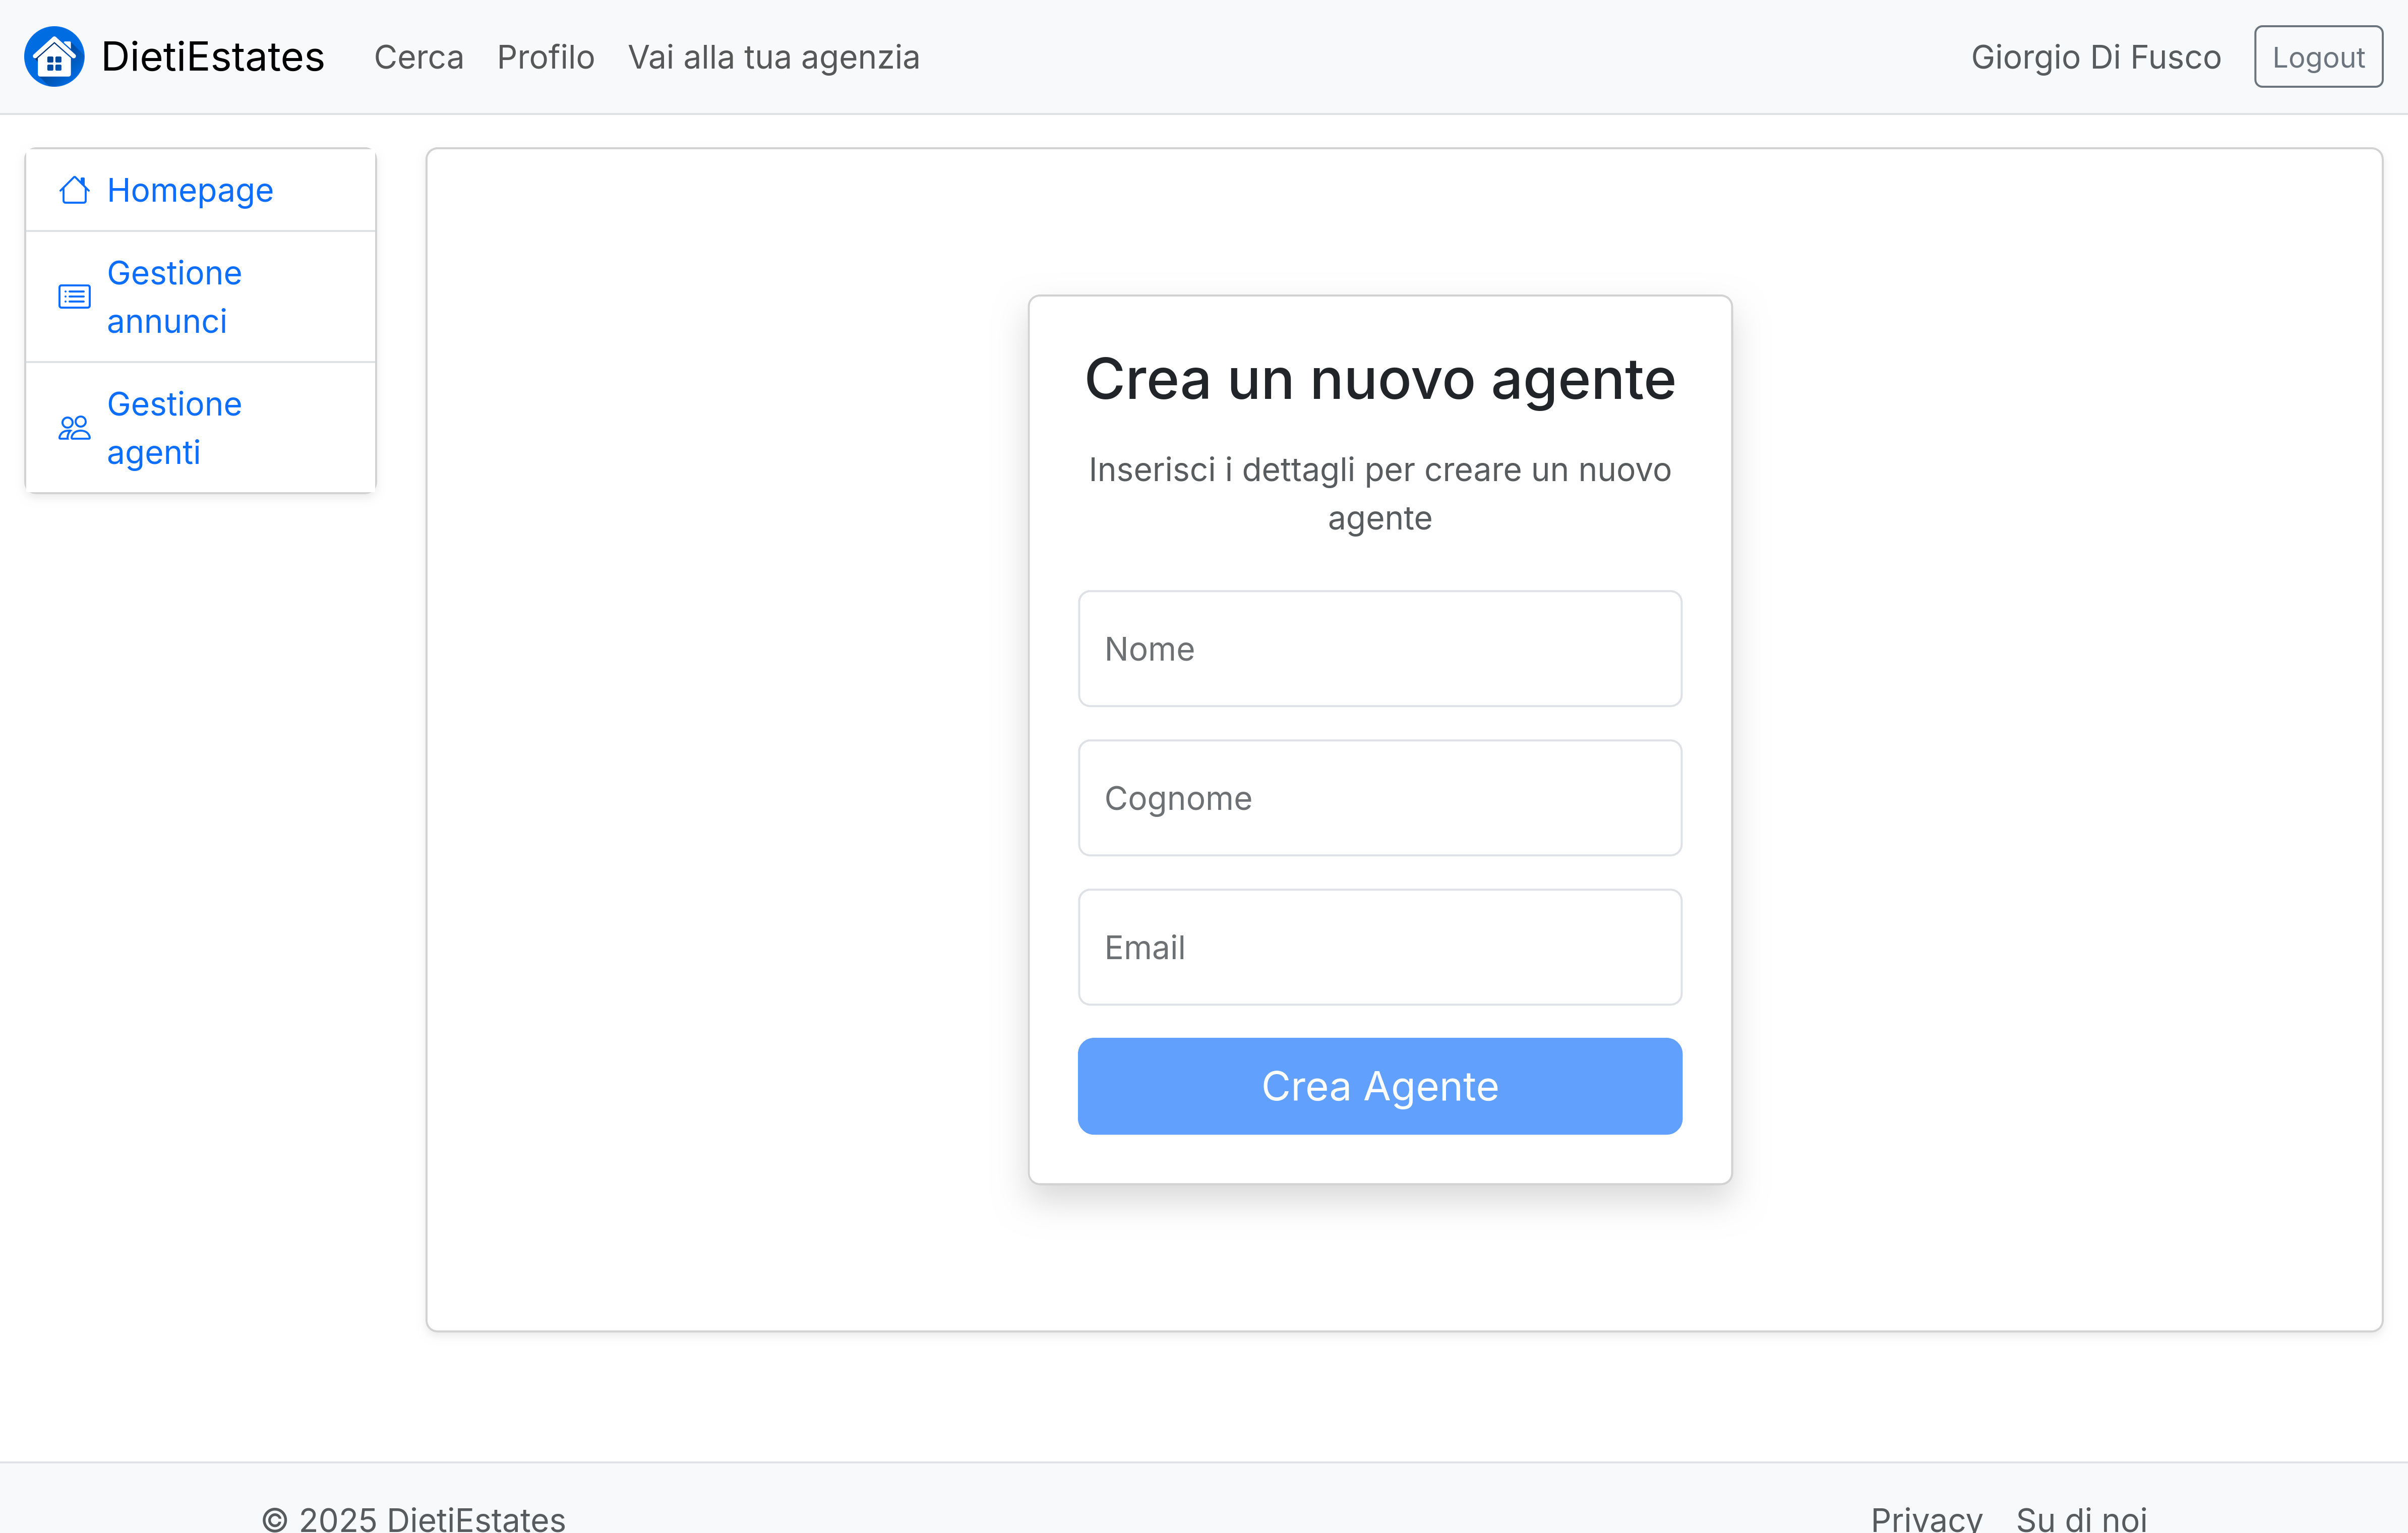
\includegraphics[width=\linewidth]{res/Mockups/agent_add.png}
	\captionof{figure}{Form aggiunta agenti immobiliari}\label{fig:add_agent}
\end{center}

\subsection{Promozione di un agente immobiliare}

\begin{longtblr}{
		width = \linewidth,
		colspec={XXXX},
		hlines,
		vlines,
	}
	\textbf{Use Case \#4} & \SetCell[c=3]{l} Promozione di un agente \\
	\textbf{Goal in Context} & \SetCell[c=3]{l} Il gestore di un'agenzia immobiliare vuole promuovere un agente \\
	\textbf{Preconditions} & \SetCell[c=3]{l} L'agente da promuovere appartiene all'agenzia \\
	\textbf{Success End Condition} & \SetCell[c=3]{l} Il collaboratore viene registrato nel sistema ed è visibile nell’elenco utenti \\
	\textbf{Failed End Condition} & \SetCell[c=3]{l} Non viene inserito alcun nuovo utente \\
	\textbf{Primary Actor} & \SetCell[c=3]{l} Gestore di una agenzia immobiliare  \\
	\textbf{Trigger} & \SetCell[c=3]{l} L'amministratore, dalla dashboard \ref{fig:dashboard_admin}, clicca su ``Promuovi'' \\
	\textbf{Main Scenario} & \textbf{Step n°} & \textbf{Agente} & \textbf{Sistema} \\
	\cline{2-3} & 1 & Seleziona la card dell'agente e clicca su ``Promuovi'' &  \\
	\cline{2-3} & 2 & & Mostra schermata di conferma. \\
	\cline{2-3} & 3 & Clicca ``Conferma'' &  \\
	\cline{2-3} & 4 & & Assegna ruolo \texttt{ROLE\_ADMIN\_ASSISTANT} all'agente  \\
	\cline{2-3} & 5 & & Invia email all'agente promosso per comunicargli della promozione \\
	\cline{2-3} & 6 & & Aggiorna la card dell'agente promosso. \\
\end{longtblr}

\begin{center}
	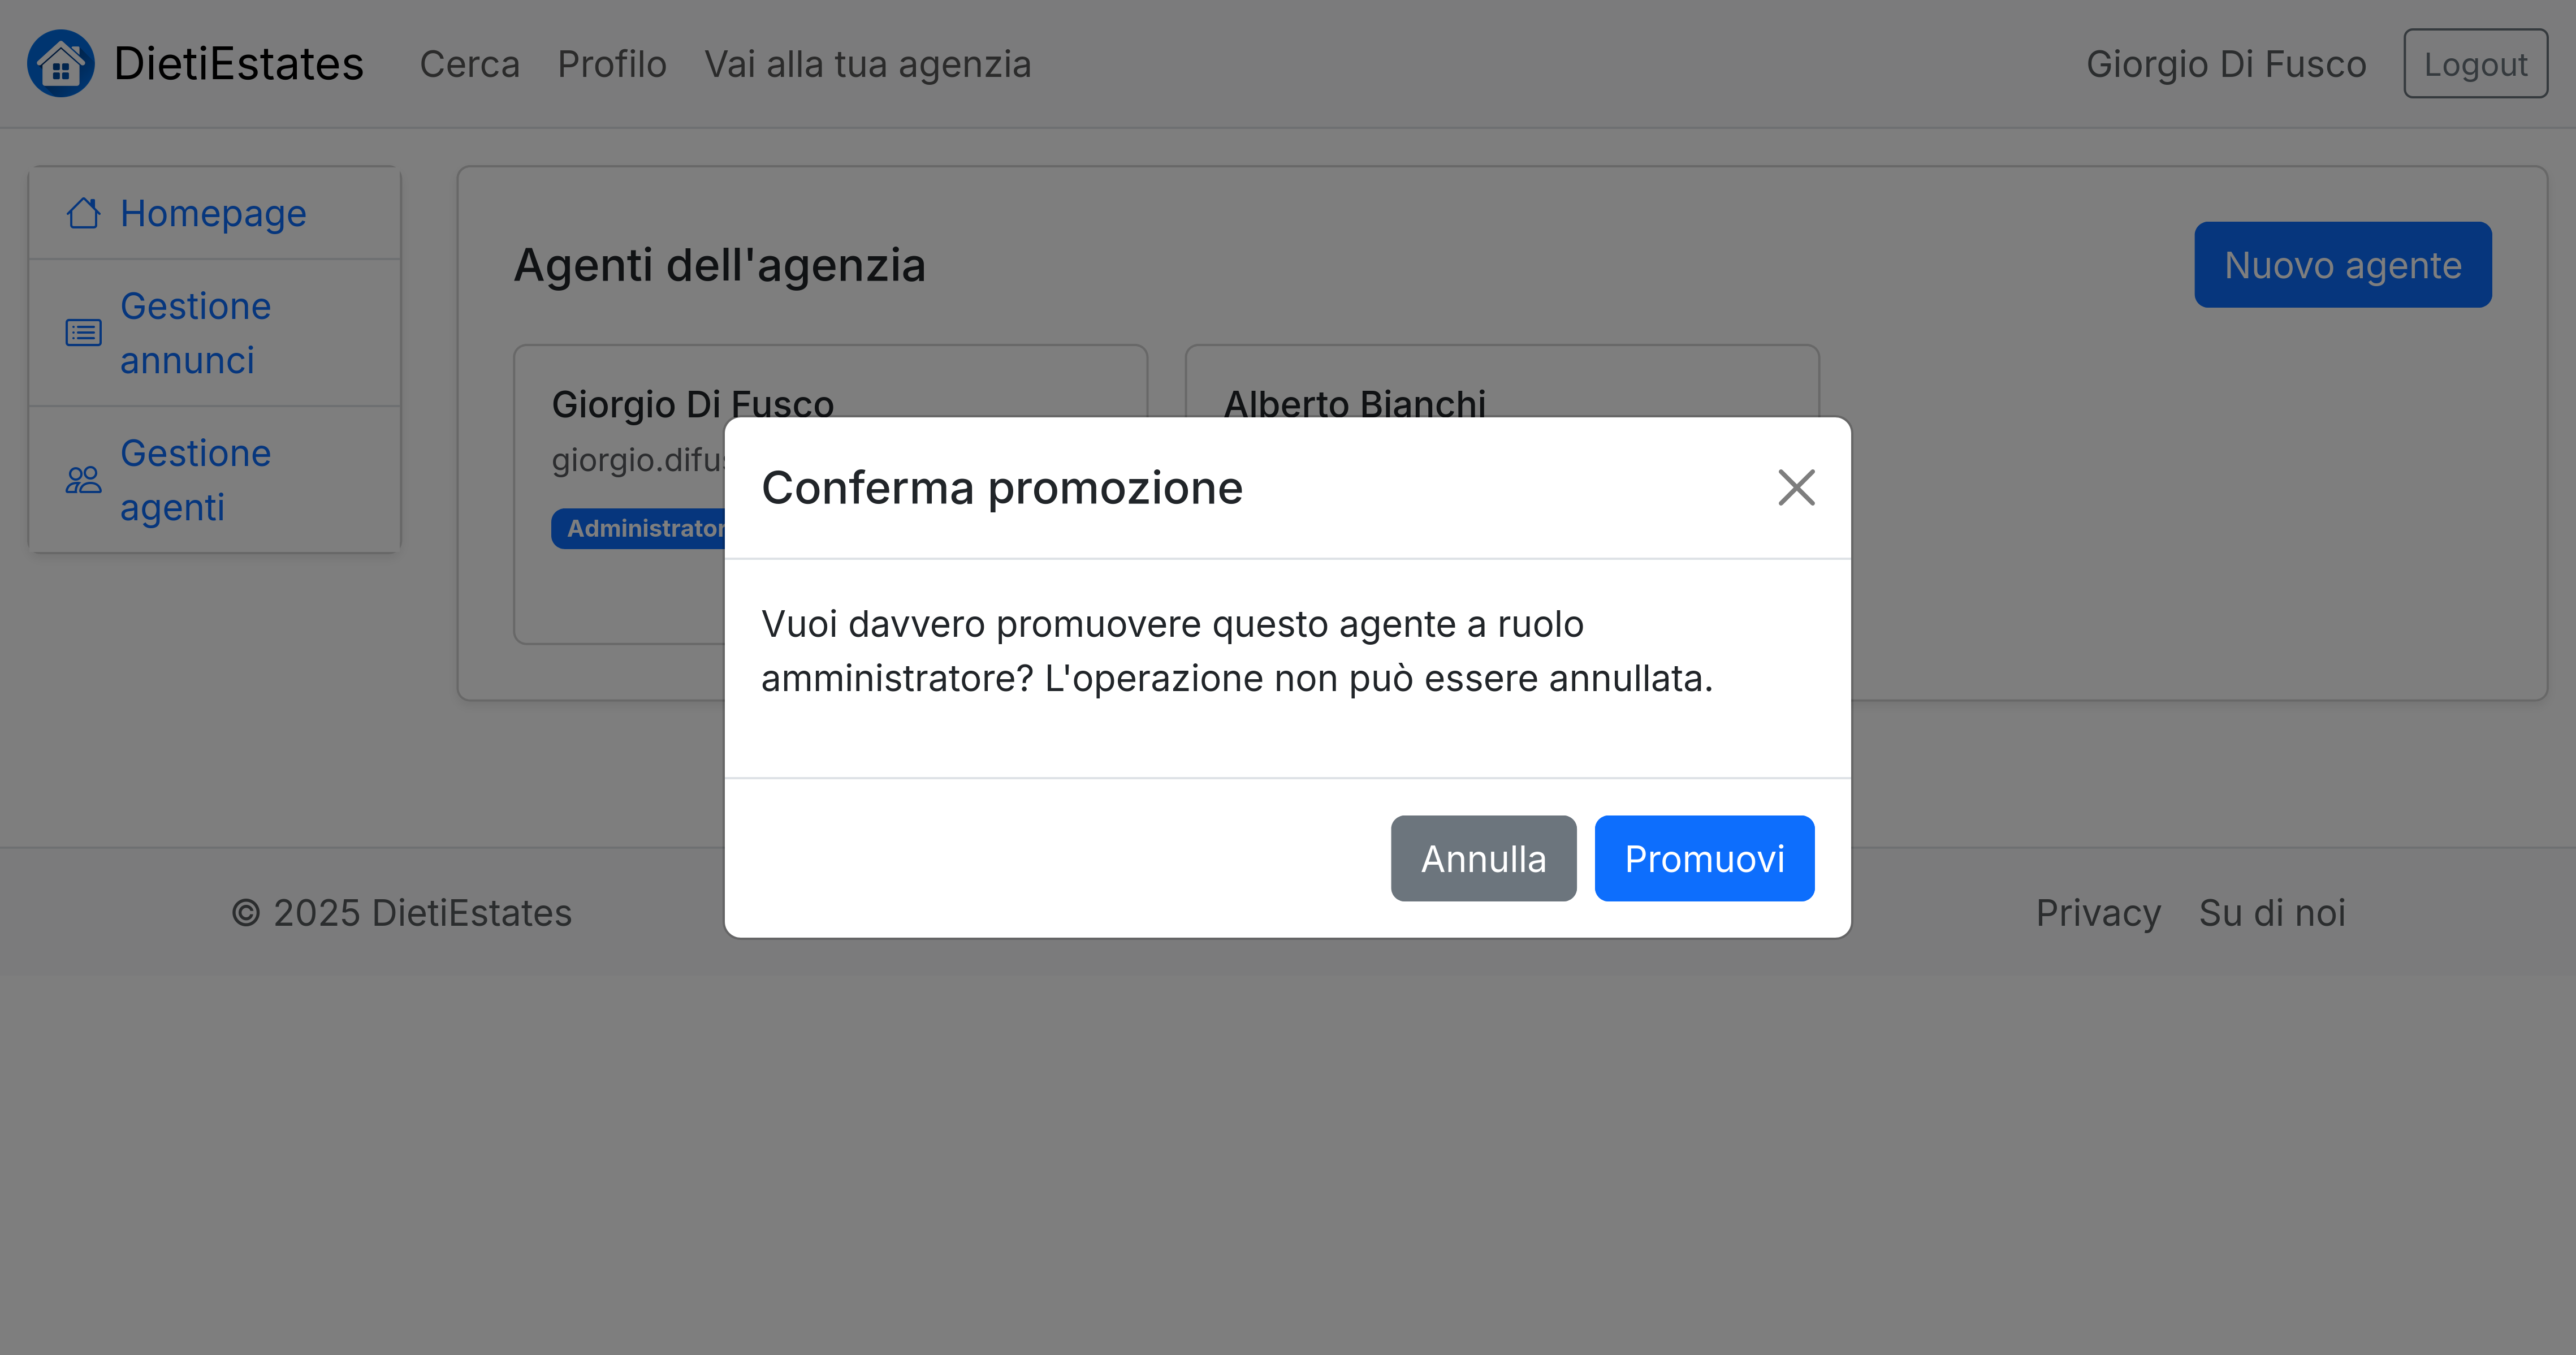
\includegraphics[width=\linewidth]{res/Mockups/promote_modal.png}
	\captionof{figure}{Finestra modale per conferma promozione}\label{fig:promote_modal}
\end{center}

\begin{center}
	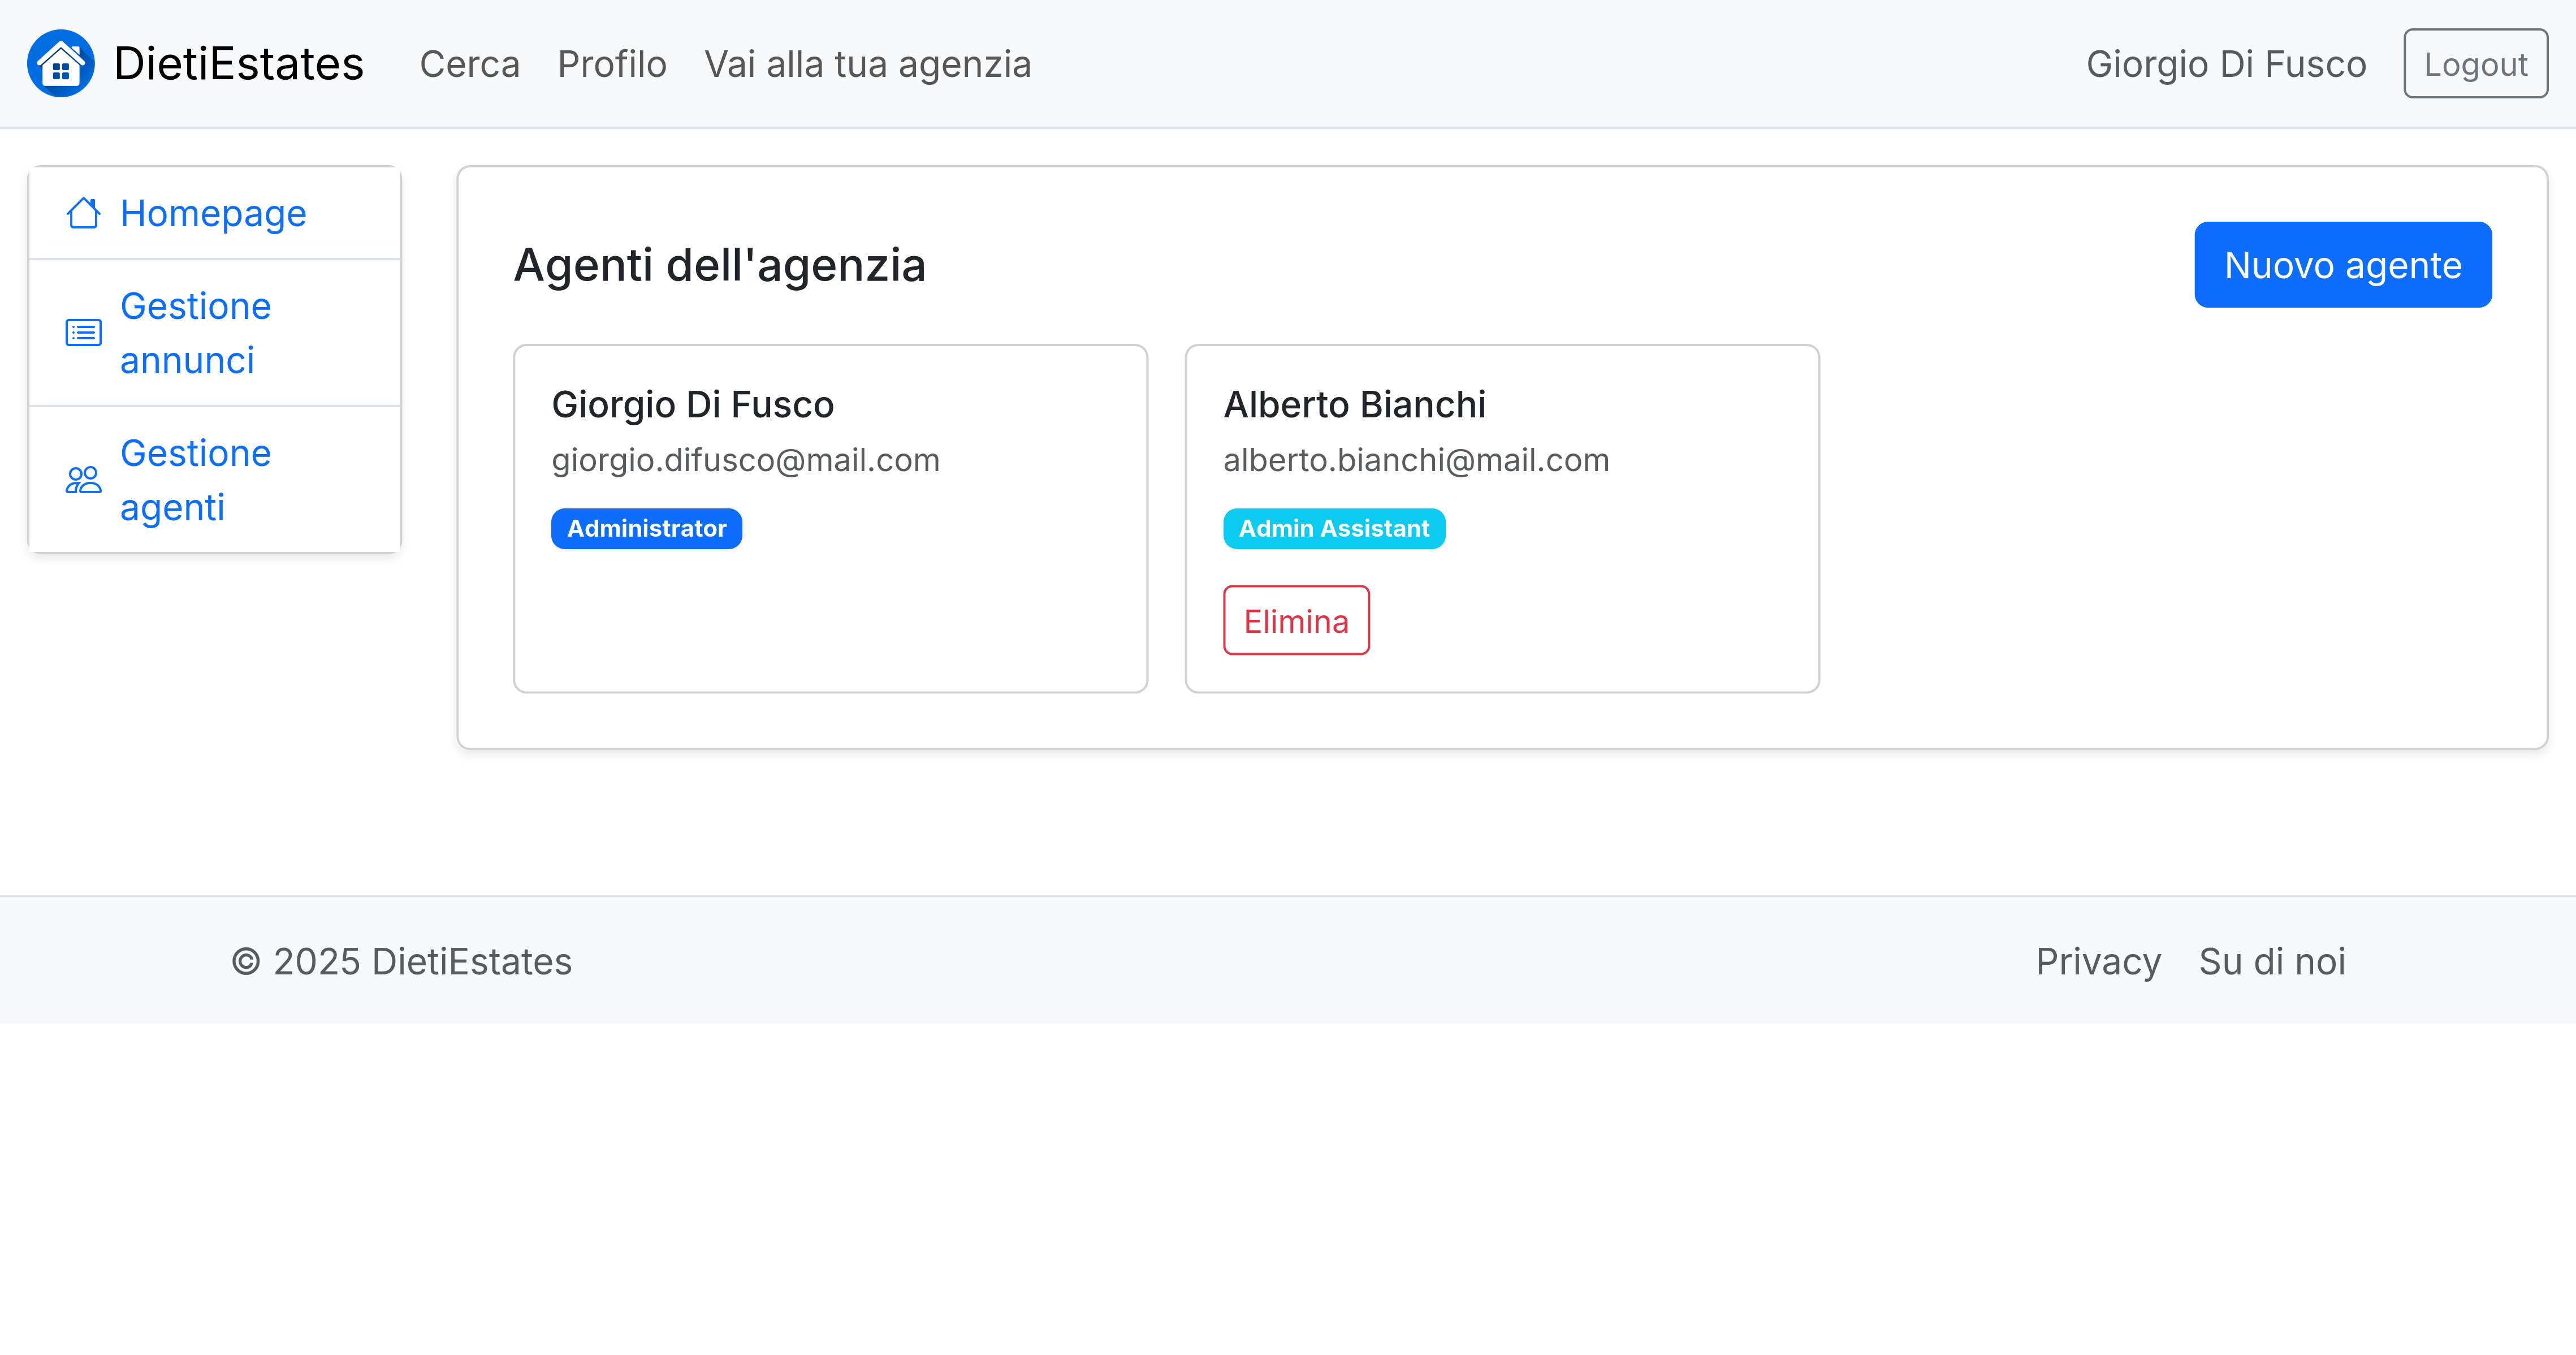
\includegraphics[width=\linewidth]{res/Mockups/agent_promoted.png}
	\captionof{figure}{Card agente aggiornata col nuovo ruolo}\label{fig:promoted_Agent}
\end{center}